\documentclass[12pt]{report}
\setcounter{secnumdepth}{3}
\setcounter{tocdepth}{3}
 
\usepackage[titletoc,toc,title]{appendix}
\usepackage[a4paper,lmargin=2.5cm,rmargin=2cm,tmargin=1cm,bmargin=1cm,includehead,includefoot]{geometry}
\usepackage[utf8]{inputenc}
\usepackage[T1]{fontenc}
\usepackage{lmodern}
\usepackage{url}
\usepackage{subcaption}
\usepackage{array}
\usepackage{amsmath}
\usepackage{amssymb}
\usepackage{mathptmx}
\usepackage{mathtools}
\usepackage{multirow}
\usepackage[scaled=.90]{helvet}
\usepackage{times}
\usepackage{wrapfig}
\usepackage{graphicx} 
\usepackage{hyperref}
\usepackage{scalefnt}
\usepackage{amsthm}
\usepackage{textcomp}
\usepackage{ragged2e}
\usepackage[section]{placeins}
\usepackage{float}
\usepackage[final]{pdfpages}
\usepackage[nobottomtitles]{titlesec}



\setlength{\emergencystretch}{2em}

\usepackage{letltxmacro}
\LetLtxMacro\origttfamily\ttfamily
\DeclareRobustCommand*{\ttfamily}{
  \origttfamily
  \hyphenchar\font=`\-\relax
  \fontdimen3\font=.25em\relax
  \fontdimen4\font=.167em\relax
  \fontdimen7\font=.167em\relax
}


\newenvironment{code}{\ttfamily}{}

\newcommand{\abs}[1]{\lvert#1\rvert}
\newcommand{\norm}[1]{\lVert#1\rVert}


\DeclareGraphicsExtensions{.jpg,.pdf,.png}
\graphicspath{{img/} {./}}

%----------------------------------------------------------------------%
\title{3D-2D Manual Registration \& Augmented Reality\\ (Project HEPATAUG)}
\author{Ismaël Tansaoui\\ \\ ALCoV - ISIT\\ Université d'Auvergne, Clermont 1\\
  \url{ismael.tansaoui8@etu.univ-lorraine.fr}\\
  \url{farqal@hotmail.fr}\\ \\
Supervisors\\  \\ Technical part: Erol Ozgur, Adrien Bartoli\\ Medical part: Emmanuel Buc, Bertrand Le Roy }

\date{\today}

\begin{document}
\maketitle


\tableofcontents


%----------------------------------------------------------------------%
\chapter{Introduction} \label{sec:introduction}

\section{Project Presentation}  \label{sec:project presentation} 
\paragraph{}
	Existing since 1980, the minimally invasive surgery is now a common practice of modern medicine. Its use is increasing because of its many advantages over open surgery. The principle of this surgery is to introduce fine surgical instruments in the patient's body, and a laparoscope which allows the surgeon to see the area on which he is operating, via small incisions of within one centimeter. The advantages of this technique for the patient are less post-operative pain, time of hospitalization and parietal scars. Nowadays, minimally invasive surgery has been frequently used in many fields such as gynecology, gastrointestinal surgery, urology, cardiovascular surgery and hepatectomy. Figure~\ref{laparoscopy} shows a scene from a minimally invasive surgery.

\paragraph{}
	The three-dimensional understanding of the surgical scene in which the surgeon operates remains a major problem. Indeed the scene filmed by the laparoscope is displayed on a screen which does not render the depth. To address this issue, an application of augmented reality on the filmed scene could allow the surgeon to be guided better.

\paragraph{}
	In a minimally invasive surgery, scanning is the only way for the surgeon to obtain information about the hidden inner topology of the organs. Technology such as computed tomography (CT) and magnetic resonance imaging (MRI) provides rich information on the body of a patient. During the surgery the laparoscope can only be placed at a short distance of the organs, so it is difficult for the surgeon to identify precisely the location of the displayed area on the organ, and therefore to know precisely the location of areas of interest, tumors for example. To address this problem, augmented reality proposes to superimpose information extracted from scanning showing the organ and its hidden topology onto the image captured by the laparoscope.

\begin{figure}[H]
\centerline{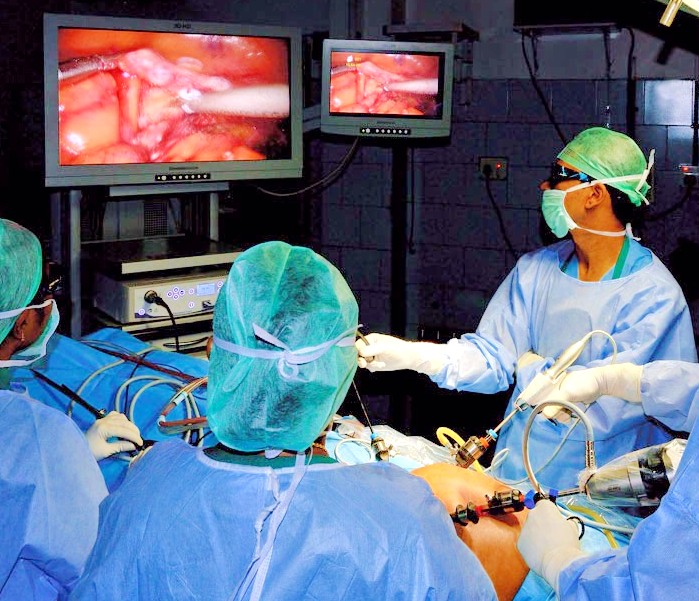
\includegraphics[scale = 0.5]{img/laparoscopy.jpg}}
\caption{A minimally invasive surgery.}
\label{laparoscopy}
\end{figure}



\section{Objectives \& Contributions} \label{sec:objectives} 

\paragraph{}
	This project will improve the quality of minimally invasive liver surgery and decrease its duration. This has a direct impact on the patient's recovery and future life. The objectives are :
\begin{enumerate}
\item To build a graphical user interface (GUI) designed with Qt, OpenGL and OpenCV in C/C++. This GUI has to be ergonomic and intuitive for the surgeons.
\item To develop a physics-based deformable model for human liver.

\item 3D-2D manual registration
\begin{enumerate}
\item Registration with rigid model
The surgeons must be able to animate the model during the surgery so that the model transposes onto the patient's liver seen from the laparoscope in a fixed pose. To do this registration, the model has to be transformed with translations and rotations. Those transformations have to be done manually through the GUI.

\item Registration with deformable model
The liver shape will change during the surgery because this is a deformable organ. So to avoid losing registration the model has to be manually deformable too. To do this registration, deformations have to be applied to the deformable model. Those deformations have to be done manually through the GUI.
\end{enumerate}

\item Augmented reality on liver
\begin{enumerate}
\item Augmentation on rigid model
By superimposing the liver model onto the real-time laparoscope video stream, surgeons will be able to see the hidden structures inside the liver for example tumors and veins. Those structures have to be fixed to the liver model. That way transformations applied to the model will also be applied to them. Then they will be visualized in their current location.

\item Augmentation on deformable model
When the liver shape changes, its inner structures position and shape can change as well. Those changes have to be calculated through the physics-based model and rendered on the screen.
\end{enumerate}
\end{enumerate}

\paragraph{}
	During my 6 months internship, I have implemented the objectives 1, 3.(a) and 4.(a).\begin{itemize}
\item GUI: The software has an ergonomic GUI, but its design has to be tested by surgeons to ensure its simplicity of use. This interface will evolve according to their feedbacks. To realize this GUI, I also designed some of its icons.

\item Rigid Registration: The software can load and display several .obj models with or without texture. They can be translated and rotated easily with the arrow keys and the mouse. Their color and opacity can be changed. The models can be saved with their transformations and textures as .obj files.

\item Augmented Reality on Rigid Model: A video stream can be displayed into the background of the scene. The liver model opacity can be adjusted so that its inner structures are visible. Their position on the displaying scene are the same as the position of the hidden structures of the patient's liver. This gives the impression of looking through a transparent liver surface.
\end{itemize}

\paragraph{}
	The remaining challenging objectives are based on the development and implementation of a deformable liver model and their inner structures. The software GUI has to be optimized by a testing process according to the feedbacks. Who is next?


\chapter{Installation of the Development Environment (1 hour 50)} \label{sec:installation of the development environment} 


\paragraph{}
This software is developed on Ubuntu 14.04.4 with the IDE Qt Creator 4.0.3 using C/C++. The libraries used are Qt 5.7, OpenGL 3.0 and OpenCV 3.1.

\section{Ubuntu installation (1 hour)}

\begin{enumerate}
\item Ubuntu 14.04.4. is used as the operating system. To install it on a computer, one must download a .iso desktop image by typing the following line in the command window:

\begin{code}
 >> wget http://releases.ubuntu.com/14.04/ubuntu-14.04.4-desktop-amd64.iso
\end{code}

\item Then the user must connect an USB key on the computer. The next command will show where the USB key is mounted (e.g. /dev/sdb).

\begin{code}
>> lsblk
\end{code}

\item We have now to unmount the USB key. The word ``PATH'' in the next command line has to be replaced by the path given in the previous step:

\begin{code}
>> sudo umount PATH
\end{code}

\item Then the computer has to be booted on the key files with the following lines:

\begin{code}
>> sudo dd if=ubuntu-14.04.4-desktop-amd64.iso of=PATH
\end{code}

\item The user can now reboot the computer. The installation interface will be launched automatically and guide the user through the installation process.
\end{enumerate}


\section{Qt librairies and Qt Creator installation (30 minutes)}
\begin{enumerate}
\item Downloading

Qt 5.7 and Qt Creator 4.0.3 can be installed by downloading the executable file ``qt-unified-linux-x64-2.0.3-1-online'' (if your Ubuntu version is 64-bit) or ``qt-unified-linux-x86-2.0.3-1-online'' (if your Ubuntu version is 32-bit) from Qt website \url{http://qt.io}.

\item File permission

Once the file downloaded, click it with the right button of the mouse and chose ``Properties''. In the tab ``Permission'', select ``Allow executing file as program'' as in the figure~\ref{qt-install-1} below. The file can now be double-clicked and will launch the setup window. Then the application will show the steps to follow.

\vspace{10pt}
\begin{figure}[H]
\centerline{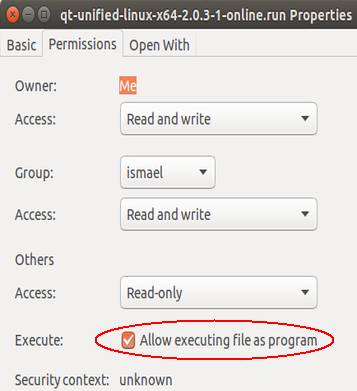
\includegraphics[scale = 0.5]{img/Qt-install-1.png}}
\caption{Properties of Qt installation file.}
\label{qt-install-1}
\end{figure}
\vspace{10pt}

\item Account creation

To install Qt, it is necessary to create an account. This can be done on the Qt website \url{http://qt.io} or by filling the form (see figure~\ref{qt-install-2} below).

\vspace{10pt}
\begin{figure}[H]
\centerline{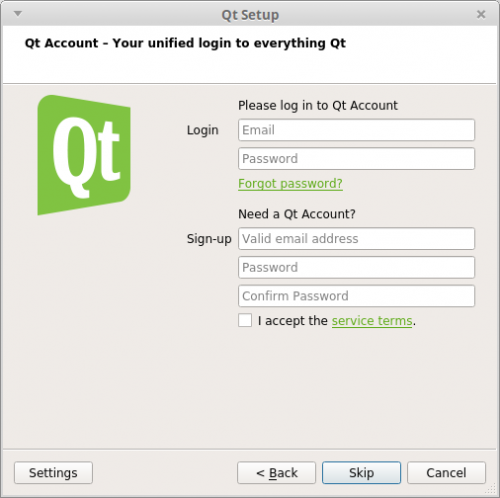
\includegraphics[scale = 0.5]{img/Qt-install-2.png}}
\caption{Register or create an account via the form.}
\label{qt-install-2}
\end{figure}
\vspace{10pt}

\item Tools selection

This step will show a check list of tools to install. It is necessary to install at least Qt 5.7 and Qt Creator, as shown on figure~\ref{qt-install-3} below.

\vspace{10pt}
\begin{figure}[H]
\centerline{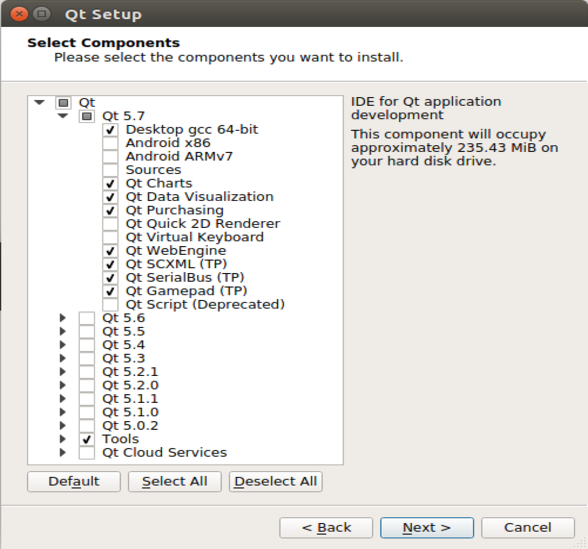
\includegraphics[scale = 0.5]{img/Qt-install-3.png}}
\caption{Selection of Qt tools to be installed.}
\label{qt-install-3}
\end{figure}
\end{enumerate}
\vspace{10pt}

\section{OpenGL librairies installation (1 minute)}
	Once Qt is installed, OpenGL must be installed as well. In order to do so, the following lines have to be typed into the terminal:

\begin{code}
>> sudo apt-get install mesa-common-dev

>> sudo apt-get install libglu1-mesa-dev
\end{code}


\section{OpenCV librairies installation (10 minutes)}
\begin{enumerate}
\item At first we need to install the dependencies required for OpenCV by typing the following lines into the terminal:

\begin{code}
>> sudo apt-add-repository ppa:mc3man/trusty-media

>> sudo apt-get update

>> sudo apt-get install ffmpeg gstreamer0.10-ffmpeg gstreamer0.10-fluendo-mp3 gstreamer0.10-gnonlin gstreamer0.10-plugins-bad-multiverse gstreamer0.10-plugins-bad gstreamer0.10-plugins-ugly totem-plugins-extra gstreamer-tools ubuntu-restricted-extras libxine1-ffmpeg gxine mencoder mpeg2dec vorbis-tools id3v2 mpg321 mpg123 libflac++6 totem-mozilla icedax tagtool easytag id3tool lame nautilus-script-audio-convert libmad0 libjpeg-progs flac faac faad sox ffmpeg2theora libmpeg2-4 uudeview flac libmpeg3-1 mpeg3-utils mpegdemux liba52-0.7.4-dev libquicktime2

>> sudo apt-get install ---assume-yes libopencv-dev build-essential cmake git libgtk2.0-dev pkg-config python-dev python-numpy libdc1394-22 libdc1394-22-dev libjpeg-dev libpng12-dev libtiff5-dev libjasper-dev libavcodec-dev libavformat-dev libswscale-dev libxine2-dev libgstreamer0.10-dev libgstreamer-plugins-base0.10-dev libv4l-dev libtbb-dev libqt4-dev libfaac-dev libmp3lame-dev libopencore-amrnb-dev libopencore-amrwb-dev libtheora-dev libvorbis-dev libxvidcore-dev x264 v4l-utils unzip
\end{code}

\item Then we have to download OpenCV:

\begin{code}
>> mkdir opencv

>> cd opencv

>> wget https://github.com/Itseez/opencv/archive/3.1.0.zip

>> unzip 3.1.0.zip
\end{code}


\item Eventually we can install OpenCV by typing the following lines:

\begin{code}
>> cd opencv-3.1.0

>> mkdir build

>> cd build

>> sudo apt install cmake

>> cmake -D CMAKE\_BUILD\_TYPE=RELEASE -D CMAKE\_INSTALL\_PREFIX=/usr/

local -D WITH\_TTB=ON -D WITH\_V4L=ON -D WITH\_OPENGL=ON -D WITH\_FFMPEG=OFF ..

>> make -j \$(nproc)

>> sudo make install

>> sudo /bin/bash -c 'echo "/usr/local/lib" >

/etc/ld.so.conf.d/opencv.conf'

>> sudo ldconfig
\end{code}
\end{enumerate}


\chapter{How to access and compile the Hepataug project using GIT (15 minutes)} \label{sec:how to access and compile the Hepataug project} 

\section{Download the project (5 minutes)}
\begin{enumerate}
\item First we have to install git:

\begin{code}
>> sudo apt-get install git
\end{code}


\item Git has to be configured for the project by typing the following lines. (Note that the email is my professional one for now but has to be changed in github settings). Replace ``path/to/project'' in the third line by the path you want for your project directory.

\begin{code}
>> git config ---global user.name "Hepataug"

>> git config ---global user.email "ismael.tansaoui8@etu.univ-lorraine.fr"

>> cd /path/to/project/

>> git init
\end{code}


\item The project files can now be downloaded from the project's Github repository \url{https://github.com/Hepataug/hepataug} by typing the following line into the terminal:

\begin{code}
>> git clone git://github.com/Hepataug/hepataug.git
\end{code}


\item The file \textbf{img.tar.gz} has to be decompressed in the release folder.
\end{enumerate}


\section{Open and compile a project (5 minutes)}
\begin{enumerate}
\item The project can finally be opened in Qt Creator (see figure~\ref{qt-install-4} below). Once Qt Creator is opened, click ``Open Project'' on the top right of the window. Then go into the folder downloaded in the previous step and open the file hepataug.pro in the window that appears.

\vspace{10pt}
\begin{figure}[H]
\centerline{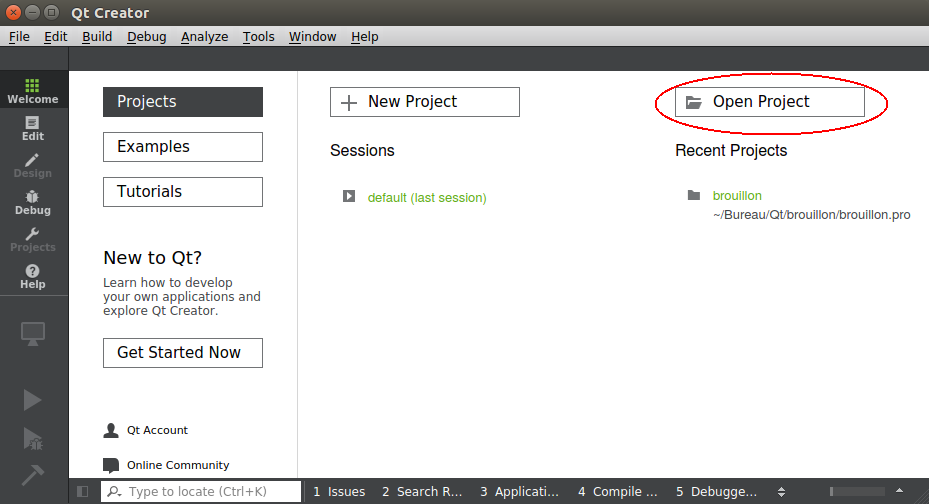
\includegraphics[scale = 0.5]{img/Qt-install-4.png}}
\caption{Qt Creator interface.}
\label{qt-install-4}
\end{figure}
\vspace{10pt}

\item Now the project can be compiled and executed by clicking the ``Run'' green arrow on the bottom left of the window (see figure~\ref{qt-install-5} below). The compilation may take one to two minutes.

\vspace{10pt}
\begin{figure}[H]
\centerline{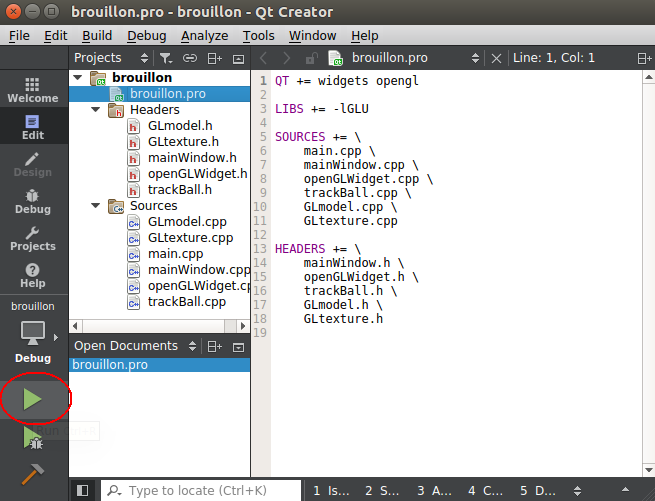
\includegraphics[scale = 0.5]{img/Qt-install-5.png}}
\caption{Opened project interface.}
\label{qt-install-5}
\end{figure}
\end{enumerate}
\vspace{10pt}

\section{Update the github repository (5 minutes)}
\paragraph{}
	When important changes are made to the software, the code has to be uploaded into the repository. That way the last version is always available for all the project members. To update the repository, one needs to type the following lines in the terminal. ``Hepataug'' is the user id and ``isit-135711'' is the password of the github account:

\begin{code}
>> cd path/to/project

>> git add ---all

>> git commit -m "COMMIT MESSAGE"

>> git push https://github.com/Hepataug/hepataug.git

>> Hepataug

>> isit-135711
\end{code}



\chapter{Tools, Theory and Key Functions} \label{sec:tools, theory and key functions}
\paragraph{}
	In this part, we will describe the software interface and features. The libraries used in this software are Qt 5.7, OpenGL 3.0 and OpenCV 3.1. Qt is used to implement the graphical user interface (GUI). OpenGL is used to draw 3D models on the screen. OpenCV is used to load videos/images and to work on them. Provided below are the links to the libraries documentation and functions :
	\begin{itemize}
	\item Qt \url{http://doc.qt.io/qt-5/}
	\item OpenGL \url{https://www.khronos.org/opengles/sdk/docs/man3/}
	\item OpenCV \url{http://docs.opencv.org/3.1.0/}
	\end{itemize}

\paragraph{}
In this chapter, we will divide the software into three parts to describe it. Firstly we will explain how the software architecture and the GUI are organized, then we will see how the models are drawn into the visual output widget and finally all the action events will be detailed.



\section{Software Architecture \& Graphical User Interface}

\paragraph{}
The architecture of the software is described in figure~\ref{diagram}. The features using Qt are colored in green, those using OpenGL in blue and the one using both OpenCV and OpenGL in red.

\begin{figure}[H]
\centerline{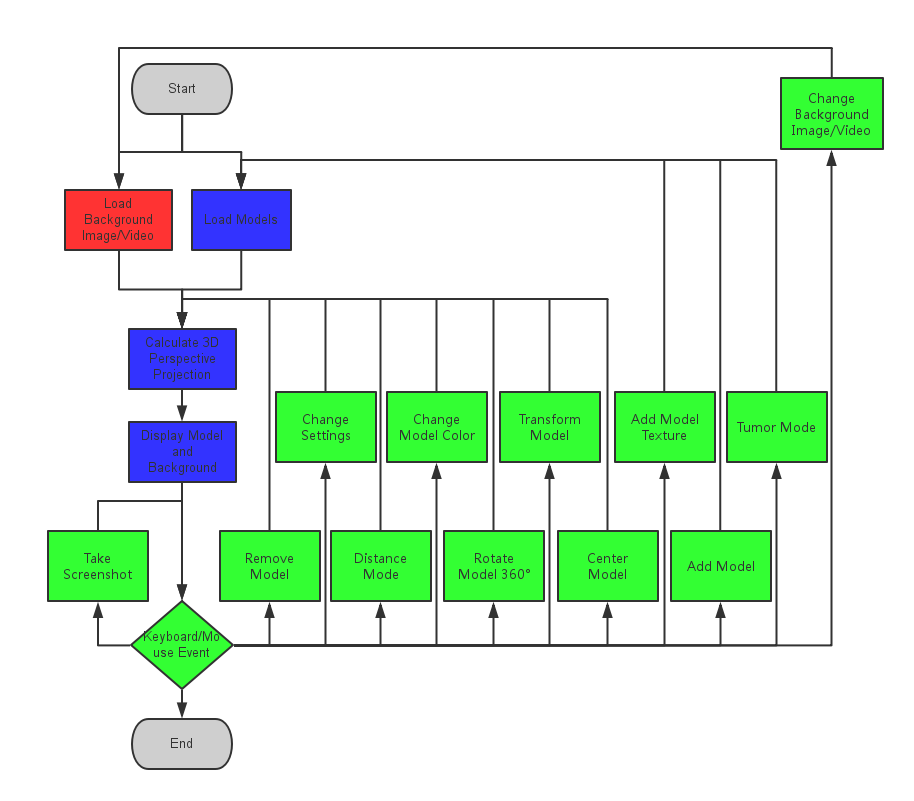
\includegraphics[scale = 0.6]{img/diagram.png}}
\caption{Hepataug software architecture.}
\label{diagram}
\end{figure}

\paragraph{}
	In figure~\ref{interface} we see the GUI. This GUI is divided into three parts. The left toolbar contains the buttons. The central visual output widget is the place where the models are drawn and moved. The right toolbar contains two sliders and the list of models uploaded.
	All the icons and images used in the GUI were found in \url{http://icones.pro/} website and some are designed.

\begin{figure}[H]
\centerline{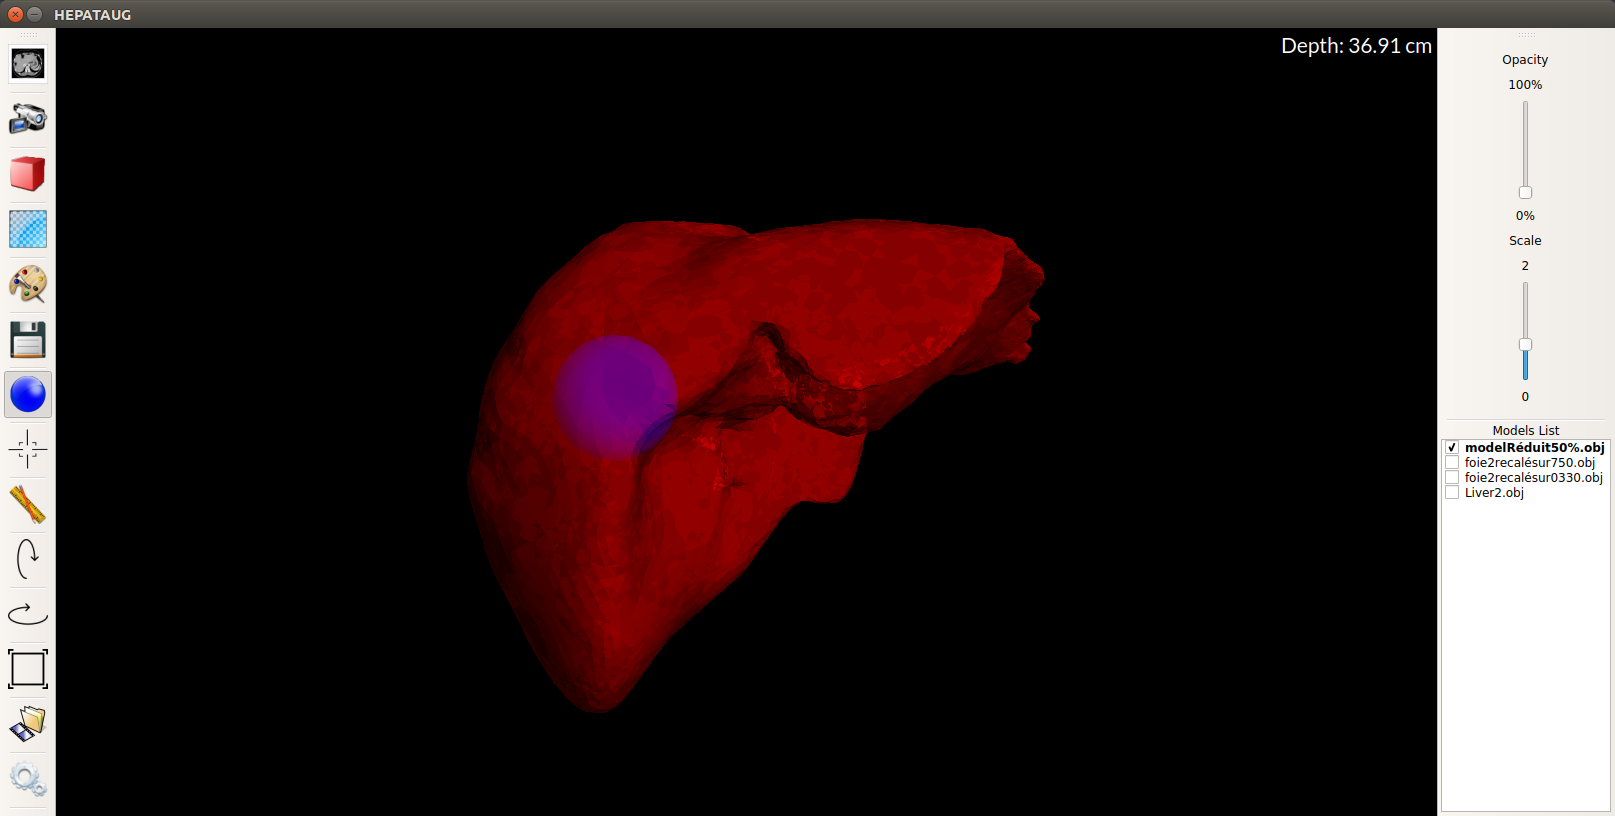
\includegraphics[scale = 0.25]{img/interface.png}}
\caption{Hepataug GUI.}
\label{interface}
\end{figure}



\section{Visual Output Widget}
\paragraph{}
	This widget displays the 3D models onto the surgical scene images. The visual output is redrawn each time the user does an action on the GUI.

\paragraph{}
	Qt inherited widget :
	\begin{code}
	QGLWidget
	\end{code}


\subsection{3D Scene Modelling}
\paragraph{}
	There are two frames; the model frame and the camera frame. The liver model points are expressed in the model frame at first. Later these points should be transformed to the camera frame so that the model is rendered correctly on the background image (see figure~\ref{perspective projection}).

\begin{figure}[H]
\centerline{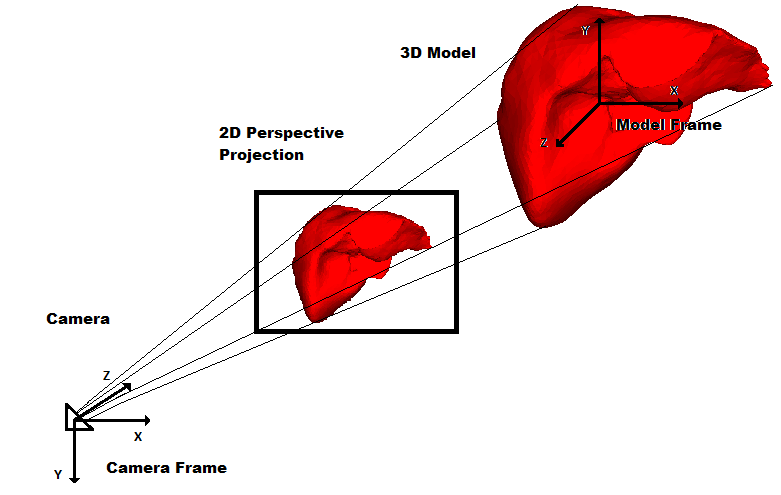
\includegraphics[scale = 0.8]{img/frame.png}}
\caption{3D scene modelling. (Note: in the code, the camera frame seen in this figure is rotated around its x-axis by 180°)}
\label{perspective projection}
\end{figure}

This GUI allows the user to perform two types of transformations; translation and rotation, which will be explained in detail in section~\ref{subsec:visual output widget}.




\subsubsection{Visual Output Rendering}
\paragraph{}
	To improve the accuracy of the registration, we want the models to be drawn as if they were displayed by the laparoscope filming the surgical scene. This is why we have to use a perspective projection with the camera parameters matrix $K$.
\begin{align}
K = \begin{pmatrix}
\alpha& s& u_0 \\
0& \beta& v_0 \\
0& 0& 1
\end{pmatrix}
\label{equ:camera parameters}
\end{align}
where
\begin{itemize}
\item $\alpha$ and $\beta$ are the focal lengths in pixels.
\item $s$ is the skewness, an artefact generated by the camera lens (unitless value).
\item $u_0$ and $v_0$ are the image center coordinates in pixels.
\end{itemize}

\paragraph{}
	To use the matrix $K$ with OpenGL, we have to rewrite it as a 4x4 matrix $\underline{K}$. The matrix (\ref{equ:implemented camera parameters}) shows how $\underline{K}$ has been implemented (Simek K., 2013 [1]):

\begin{align}
\underline{K} = \begin{pmatrix}
\alpha& s& -u_0& 0 \\
0& \beta& -v_0& 0 \\
0& 0& A& B\\
0& 0& -1& 0
\end{pmatrix}
\label{equ:implemented camera parameters}
\end{align}
where $A = near + far$ and $B = near \times far$, with $near$ and $far$ being the minimal and maximal distances in meters for the model to be displayed, respectively.

\paragraph{}
	Perspective projection is calculated with this new $\underline{K}$ matrix and the transformation matrix $T$ between the model frame and the camera frame. $T$ is computed by OpenGL automatically. With this projection matrix applied on the models, they can be correctly visualized with the real liver image in the background.


\paragraph{}
	OpenGL functions :

	\begin{code}
	glMatrixMode(GL\_PROJECTION), glOrtho, glMultMatrixf
	\end{code}


\subsubsection{Z-buffer}
\paragraph{}
	By default, the faces of the models are displayed in the order they are called in the code. This system does not render depth properly because the last drawn models will always be in front of the other ones, regardless their depth. To solve this problem, we use the OpenGL Z-buffer. This buffer is a two-dimensioned table and each cell represents a screen pixel in which the $z$ value of the displayed model surface is stored. When two model surfaces are displayed in the same pixel, the buffer compares their $z$ value (the distance from the camera) and only displays the one having the lower value.
	In order for the background to always be displayed behind the models, the Z-buffer is temporarily disabled when the background is drawn.

\paragraph{}
	OpenGL functions :

	\begin{code}
	glEnable(GL\_DEPTH\_TEST), glDisable(GL\_DEPTH\_TEST)
	\end{code}
 


\subsection{Measurement Informations}
\paragraph{}
	When only one model is active, we can see the depth of the model center at the top-right of the widget (number 3 on figure~\ref{centralwidget}). If the distance mode is active (see subsection~\ref{subsubsec:distance mode}), we can read the distance between the two tags at the top-right of the widget (number 4). If we left-click on the model, a cross will be drawn on the surface of the model. Then the coordinates of the screen point (in $px$) and of the selected surface point (in $cm$) will be displayed at the top-left (number 1 and 2). If the tumor mode is active (see subsection~\ref{subsubsec:tumor mode}), the distance between this point and the tumor center will be displayed at the bottom-left (number 5) using the formula (\ref{equ:norm}) (subsection~\ref{subsubsec:crosshair}).

\begin{figure}[H]
\centerline{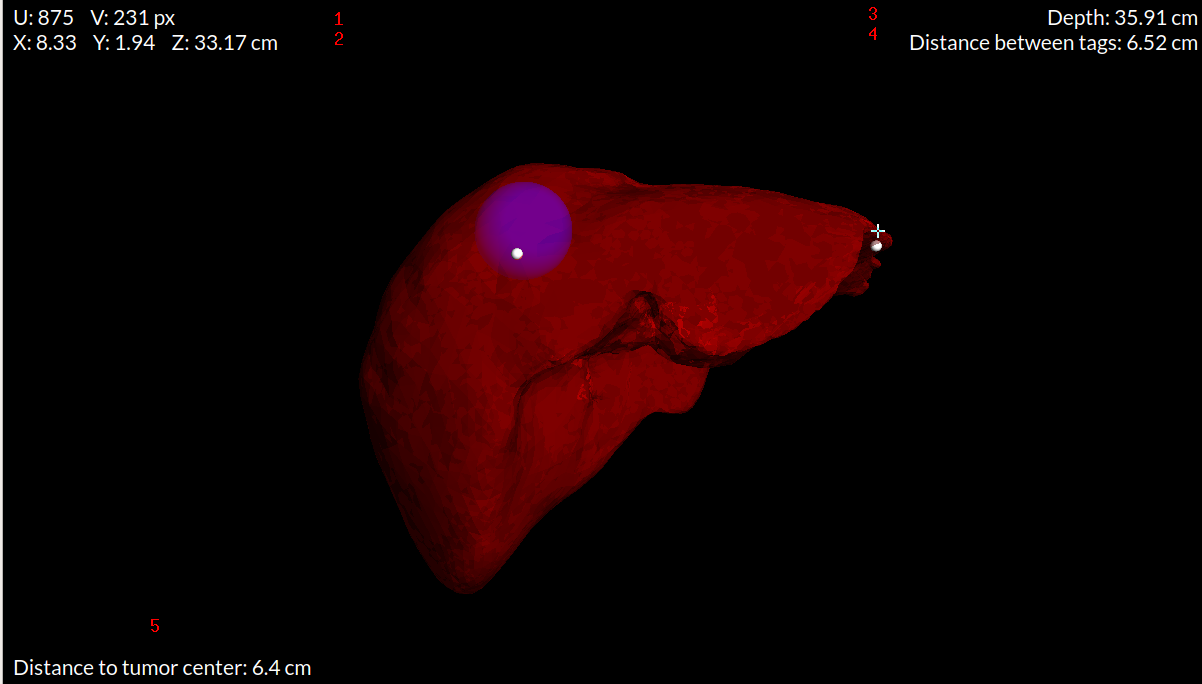
\includegraphics[scale = 0.3]{img/centralWidget.png}}
\caption{Visual output widget elements}
\label{centralwidget}
\end{figure}

\paragraph{}
	Developed functions :

	\begin{code}
	OpenGLWidget -> paintGL, createCrosshair, mousePressEvent
	\end{code}

\paragraph{}
	Qt functions :

	\begin{code}
	QGLWidget -> renderText
	\end{code}

\paragraph{}
	OpenGL functions :

	\begin{code}
	glLogicOp, glCallList, glColor4f
	\end{code}




\section{Action Events} \label{sec:action events}
\paragraph{}
	This section will describe the interactions between the user and the GUI. Those actions will be grouped according to how they are activated from the GUI. They can be activated from keyboard and mouse in the visual output widget, from the left toolbar buttons or from the right toolbar sliders and models list. The visual output widget is updated every time an action event is performed by the user.



\subsection{Visual Output Widget Interaction} \label{subsec:visual output widget}
\paragraph{}
	When this widget is active, the chosen models can be translated and rotated. Those transformations and how to perform it are described bellow.
Pressing the ``Escape'' key quits the software.


\subsubsection{Translation}
\paragraph{}
	A translation can be performed on the chosen models with the arrow keys and the mouse wheel. The keys ``Left'' and ``Right'' move the model in $x$ axis, ``Top'' and ``Bottom'' in $y$ axis and the mouse wheel in $z$ axis of the camera frame. If ``Ctrl'' is pressed at the same time, then a fine translation can be performed. By default, each arrow key pressed or mouse wheel step rolled moves the active models of $1 cm$ on the chosen axis and the fine translation moves them of $0.1 cm$.


\paragraph{}
	The translation moves every point of a model by the same amount. This translation can be represented by $t=(a, b, c, 0)^{\top}$, an homogeneous vector. To obtain the point $p'=(x', y', z', 1)^{\top}$ from a translation $t$ of the point $p=(x, y, z, 1)^{\top}$, we have to add the $p$ point coordinates with the translation vector $t$:
\begin{gather}
p' = p + t
\end{gather}


\paragraph{}
	Developed functions :

	\begin{code}
	OpenGLWidget -> wheelEvent, keyPressEvent
	\end{code}

\paragraph{}
	OpenGL functions :

	\begin{code}
	glTranslatef
	\end{code}


\subsubsection{Rotation}	\label{subsubsec:rotation}
\paragraph{}
	Performing a drag and drop with the mouse left button on the visual output widget rotates chosen models around their own central model frame (see figure~\ref{rotation}). The user can define a reference frame among the models in the right toolbar models list. This model will appear in bold in the list. If a model's frame is selected as a reference frame, all the translations applied to it will also be applied to the other models. The other models' rotations will also be performed around the reference frame instead of their own frames. The purpose of this feature is to be applied to the liver. When the liver is the reference frame, all the other models as tumors and veins will follow its translations and rotations.

\begin{figure}[H]
\centerline{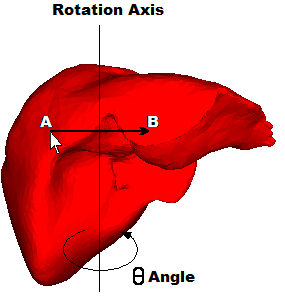
\includegraphics[scale = 1]{img/rotation.png}}
\caption{Representation of the rotation axis and angle when the cursor is dragged from a pixel $A$ to a pixel $B$.}
\label{rotation}
\end{figure}

\paragraph{}
	 The formulas used in this part are based on the ones found in this website: \url{http://pages.cpsc.ucalgary.ca/~tfalders/CPSC453/Trackball.png}. The rotation is a circular movement of an object around an imaginary line called a rotation axis. In the following example we will rotate an $p=(x, y, z, 1)^\top$ point around the $(a, b, c)$ axis by an angle $\theta$ in $radians$. To obtain the new point $p'$ coordinates, we have to multiply the $p$ point coordinates with a rotation matrix $R$ containing those parameters. Let $C = cos(\theta)$ and $S = sin(\theta)$, then $R$ is defined as:

\begin{gather}
R = \begin{pmatrix}
a^2(1-C) + C&   ab(1-C) - c \times S& ac(1-C) + b \times S& 0\\
ba(1-C) + c \times S& b^2(1-C) + C&   bc(1-C) - a \times S& 0\\
ac(1-C) - b \times S& bc(1-C) + a \times S& c^2(1-C) + C& 0\\
0& 0& 0& 1
\end{pmatrix}
\end{gather}

\paragraph{}
	and $p'$ as :

\begin{gather}
p' = R p
\end{gather}


\paragraph{Drag and drop with mouse:}
	When the user moves the mouse from an $A=(x,y)^\top$ point to a $B=(x',y')^\top$ point, he expects the model to rotate around a $N$ axis orthogonal to the plane defined by vectors $L_{previous}=(x,y,z)^\top$ and $L_{current}=(x',y',z')^\top$. The main difficulty in order to implement the rotation interface with the mouse is that we need the object to rotate in 3D and the cursor can only move in 2D. To address this problem, the software calculates a $z$ coordinate from $x$ and $y$ and a $z'$ coordinate from $x'$ and $y'$. When the user clicks the widget to perform a rotation, the cursor pixel coordinates of $A$ are saved. The formula used to calculate $z$ has been designed to allow the user to have a sense of depth as he rotates models:

\begin{gather}
z = 1 - \norm{\left( \begin{array}{cc}
x \\
y \end{array} \right)}
\end{gather}

\paragraph{}
	From those coordinates we create the 3D vector $L=(x,y,z)^\top$, stored into the memory. Then the user will move the mouse. The new position is saved into $B$ and the same formula as above is used to calculate a new $L$ vector.
	Now that we have two 3D vectors $L_{previous}$ and $L_{current}$ we can calculate the rotation axis. To calculate $N$, we use a cross product between those two vectors:
\begin{gather}
N = L_{previous} \times L_{current}
\end{gather}

\paragraph{}
The rotation angle $\theta$ (in $degrees$) is function of the $arcsin$ of the vector $N$ $length$ because this gives a better accuracy for the user than a linear function.

\begin{gather}
\theta = \frac{180}{\pi} arcsin(\norm{N})
\label{equ:angle}
\end{gather}

\paragraph{}
Each model has a quaternion to indicate its rotation from its own frame. This quaternion $Q~=~(X,Y,Z,W)^{\top}$ is calculated from the axis $N=(a,b,c)^{\top}$ and the angle $\theta$. A quaternion which represents a general rotation can be interpreted geometrically as follows: 

\begin{align}
Q = \left( \begin{array}{cc}
X \\
Y \\
Z \\
W \end{array} \right)
= \left( \begin{array}{cc}
a * sin\left(\frac{\theta}{2}\right) \\
b * sin\left(\frac{\theta}{2}\right) \\
c * sin\left(\frac{\theta}{2}\right) \\
cos\left(\frac{\theta}{2}\right)^{2} \end{array} \right)
\end{align}

\paragraph{}
	For the quaternion $Q$, the corresponding homogeneous rotation matrix $R_Q$ is defined as follows (Shoemake K., 1985 [2]):

\begin{align}
R_Q = \begin{pmatrix}
1-2Y²-2Z²& 2WY+2WZ& 2XZ-2WY& 0\\
2XY-2WZ& 1-2X²-2Z²& 2YZ+2WX& 0\\
2XZ+2WY& 2YZ-2WX& 1-2X²-2Y²& 0\\
0& 0& 0& 1
\end{pmatrix}
\end{align}

\paragraph{}
	The calculations to obtain $Q$ from $N$ and $\theta$, and the one to obtain $R_Q$ from $Q$ are done automatically by OpenGL functions.





\paragraph{}
	Developed functions :

	\begin{code}
	OpenGLWidget -> mousePressEvent, mouseMoveEvent, multMatrix
	
	TrackBall -> push, move
	\end{code}

\paragraph{}
	Qt functions :

	\begin{code}
	QTime -> currentTime, msecsTo

	QQuaternion -> fromAxisAndAngle

	QMatrix4x4 -> rotate, transposed

	QVector3D -> crossProduct, normalize, length
	\end{code}

\paragraph{}
	OpenGL functions :

	\begin{code}
	glMultMatrixf
	\end{code}


\subsubsection{Get Point Coordinates} \label{subsubsec:crosshair}
\paragraph{}
	A left-click on the surface of a model creates a crosshair at the clicked location. Then the coordinates of the screen coordinates at this point are displayed in $px$ at the top-left of the widget. The coordinates of the model point ``under'' the crosshair are displayed as well in $cm$.


\paragraph{}
	Developed functions :

	\begin{code}
	OpenGLWidget -> createCrosshair, mousePressEvent,

	screenToModelPixel
	\end{code}

\paragraph{}
	Qt functions :

	\begin{code}
	QGLWidget -> renderText
	\end{code}

\paragraph{}
	OpenGL functions :

	\begin{code}
	glLoadIdentity, glOrtho,  glGenLists, glNewList, glEndList,
	
	glLogicOp, glCallList, glColor4f
	\end{code}





\subsection{Left Toolbar Buttons} \label{subsec:left toolbar}
\paragraph{}
This subsection shows the buttons of the left toolbar. We will explain their function and implementation.

\subsubsection{Load Image}

\begin{wrapfigure}[3]{l}{1.5cm}
\vspace{-20pt}
\includegraphics[width=1.5cm]{icons/picture.jpg}
\end{wrapfigure}
\paragraph{}
	This button opens an explorer window for the user to select an image file. This image will be loaded, converted into an OpenGL matrix and displayed in the central visual output widget as a background. The GUI will be automatically resized to fit the new image.

\paragraph{}
	Developed functions :

	\begin{code}
	OpenGLWidget -> setTexturePath
	
	GLtexture -> setTexture(QString)
	\end{code}

\paragraph{}
	Qt functions :

	\begin{code}
	QFileDialog -> getOpenFileName

	QImage -> width, height

	QGLWidget -> convertToGLFormat
	\end{code}

\paragraph{}
	OpenGL functions :

	\begin{code}
	glGenTextures, glBindTexture, glTexImage2D, glTexParameteri
	\end{code}



\subsubsection{Load Video} \label{subsubsec:load video}

\begin{wrapfigure}[3]{l}{1.5cm}
\vspace{-20pt}

\includegraphics[width=1.5cm]{icons/camera.png}
\end{wrapfigure}
\paragraph{}
	This button opens an explorer window for the user to select a video file. A timer is started to read each frame one by one and redraw the scene every $\frac{1}{fps}$ seconds. The value of $fps$ (frame per second) is read from the video file. This video will be displayed in the central visual output widget as a background. The GUI will be automatically resized to fit the video.

\paragraph{}
	Developed functions :

	\begin{code}
	OpenGLWidget -> setVideoPath

	GLtexture -> setTexture(Mat)
	\end{code}

\paragraph{}
	Qt functions :

	\begin{code}
	QFileDialog -> getOpenFileName

	QTimer -> start, stop

	QImage -> width, height

	QGLWidget -> convertToGLFormat
	\end{code}

\paragraph{}
	OpenCV functions :

	\begin{code}
	VideoCapture -> get(CAP\_PROP\_FPS), release

	Mat -> cvtColor, bits
	\end{code}

\paragraph{}
	OpenGL functions :

	\begin{code}
	glGenTextures, glBindTexture, glTexImage2D, glTexParameteri
	\end{code}



\subsubsection{Load Model}

\begin{wrapfigure}[3]{l}{1.5cm}
\vspace{-20pt}

\includegraphics[width=1.5cm]{icons/load.png}
\end{wrapfigure}
\paragraph{}
	This button opens an explorer window for the user to select an object file (.obj). This file is read by the software parser to create the OpenGL vertices and faces. The created model is stored in a display list to save RAM, so that it does not have to be redrawn each time the scene is updated. If the file contains texture coordinates and a texture path, the texture is loaded. If the .obj file does not contain the normal of the polygons (triangles or quadrilateral), the normal vector $V_n$ of a polygon is automatically calculated with this formula:

	\begin{align}
	V_n = \frac{\vec{AB} \times \vec{AC}}{\norm{\vec{AB} \times \vec{AC}}}
	\end{align}

\paragraph{}
	where $A, B, C$ are three polygon points.

\paragraph{}
	The normal vectors are necessary for the light and shadows to be applied correctly on each polygon. Those nuances of shadow are a key element in the perception of the depth of the model surface (see figures~\ref{modelwithoutshadows} and \ref{modelwithshadows}).

\begin{figure}[H]
\minipage{0.5\textwidth}
\centerline{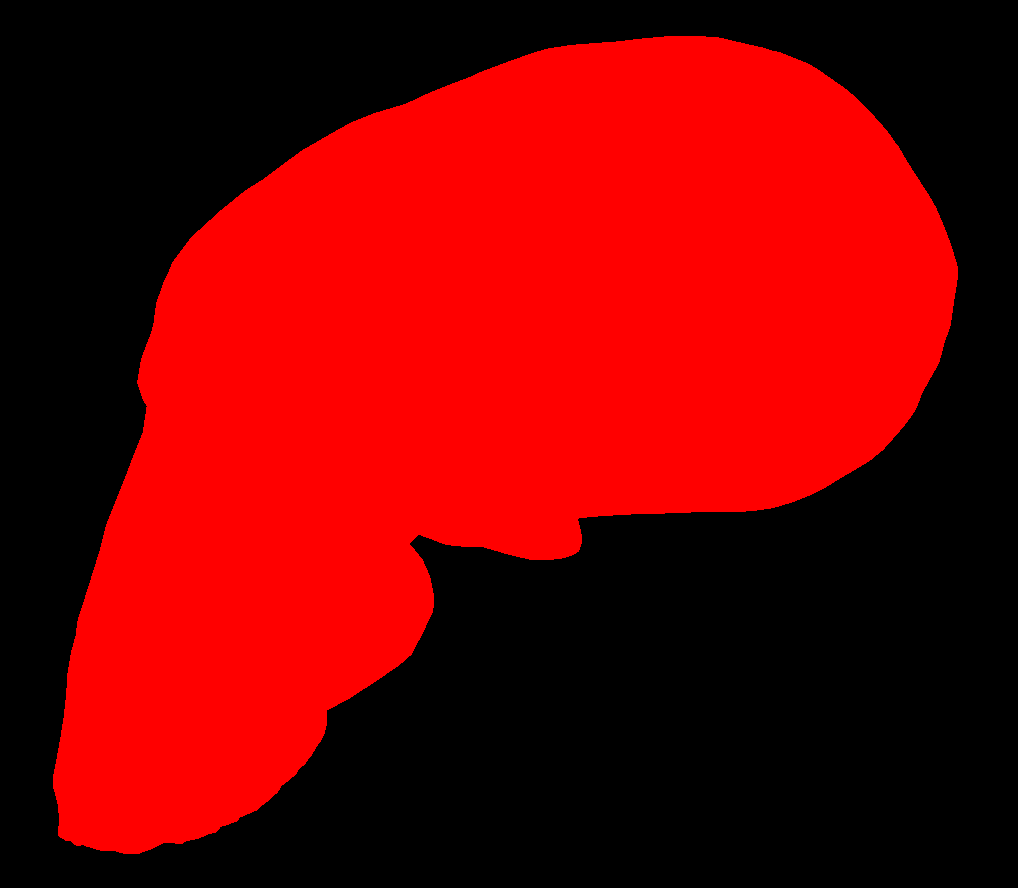
\includegraphics[scale = 0.3]{img/modelWithoutShadows.png}}
\caption{Model without shadows.}
\label{modelwithoutshadows}
\endminipage\hfill
\minipage{0.5\textwidth}
\centerline{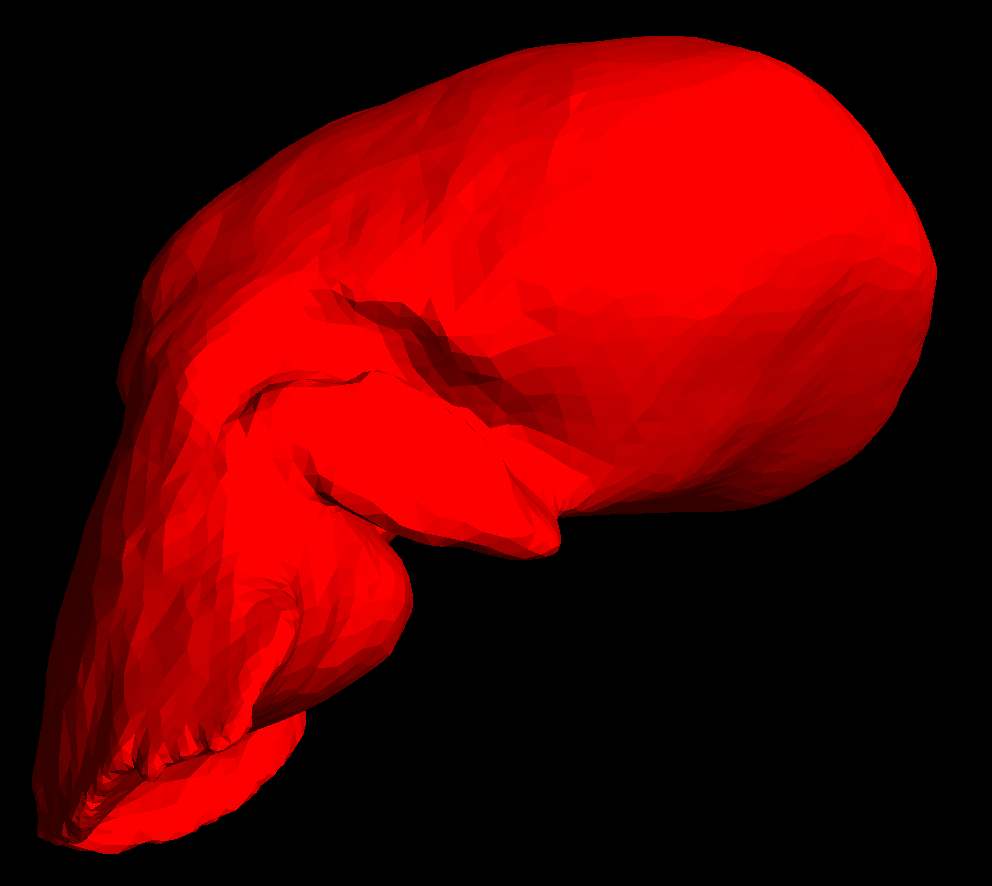
\includegraphics[scale = 0.3]{img/modelWithShadows.png}}
\caption{Model with shadows.}
\label{modelwithshadows}
\endminipage
\end{figure}


\paragraph{}
	The model then will be added to the central visual output widget and its name will be added to the model list on the right toolbar.


\paragraph{}
	Developed functions :

	\begin{code}
	OpenGLWidget -> addModel

	GLmodel -> loadModel, calculateNormal, drawFace, loadMTL,

	loadTexture
	\end{code}

\paragraph{}
	Qt functions :

	\begin{code}
	QFileDialog -> getOpenFileName

	QFile -> open, close

	QTextStream -> atEnd, readLine

	QGLWidget -> convertToGLFormat
	\end{code}

\paragraph{}
	OpenGL functions :

	\begin{code}
	glNewList, glBegin, glEnd, glEndList, glNormal3f, glTexCoord2f,

	glVertex3f, glGenTextures, glBindTexture, glTexImage2D,

	glTexParameteri
	\end{code}



\subsubsection{Load Texture}

\begin{wrapfigure}[3]{l}{1.5cm}
\vspace{-20pt}

\includegraphics[width=1.5cm]{icons/texture.png}
\end{wrapfigure}
\paragraph{}
	This button opens an explorer window for the user to select an image file. This image will be textured on all active models. If the model file contains texture coordinates, the texture will be drawn once on all the model surface. If the model files did not contain texture coordinates, the texture will be drawn repetitively on each model polygon.

\paragraph{}
	Developed functions :

	\begin{code}
	OpenGLWidget -> addTexture

	GLmodel -> loadTexture
	\end{code}

\paragraph{}
	Qt functions :

	\begin{code}
	QFileDialog -> getOpenFileName

	QGLWidget -> convertToGLFormat
	\end{code}

\paragraph{}
	OpenGL functions :

	\begin{code}
	glGenTextures, glBindTexture, glTexImage2D, glTexParameteri
	\end{code}



\subsubsection{Change Color}

\begin{wrapfigure}[2]{l}{1.5cm}
\vspace{-20pt}

\includegraphics[width=1.5cm]{icons/color.png}
\end{wrapfigure}
\paragraph{}
	This button opens a color palette window for the user to select a new color (see figure~\ref{changecolor}). This color will be applied to all active models.

\begin{figure}[H]
\centerline{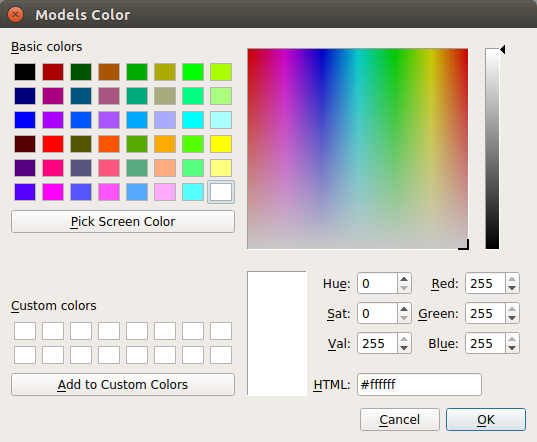
\includegraphics[scale = 0.5]{img/changeColor.png}}
\caption{Color palette window.}
\label{changecolor}
\end{figure}

\paragraph{}
	Developed functions :

	\begin{code}
	ModelsListWidget -> emitChangeColor
	
	OpenGLWidget -> changeColor
	\end{code}

\paragraph{}
	Qt functions :

	\begin{code}
	QColorDialog -> getColor

	QColor -> redF, blueF, greenF
	\end{code}



\subsubsection{Save Models}

\begin{wrapfigure}[3]{l}{1.5cm}
\vspace{-20pt}

\includegraphics[width=1.5cm]{icons/save.png}
\end{wrapfigure}
\paragraph{}
	This button opens an explorer window for the user to select folder and type a name for a new .obj file. The model vertices, faces, normal, path, coordinates and texture coordinates are written in the new file, after applying the current models transformations. If several models are active, a dialog box requires the user to indicate whether he wants to merge the models in one or to save them individually in different files.

\paragraph{}
	Developed functions :

	\begin{code}
	OpenGLWidget -> saveModels

	GLmodel -> saveModel
	\end{code}

\paragraph{}
	Qt functions :

	\begin{code}
	QFileDialog -> getSaveFileName

	QMessageBox -> exec

	QFile -> open, close

	QTextStream -> fluxOut
	\end{code}



\subsubsection{Add Tumor} \label{subsubsec:tumor mode}

\begin{wrapfigure}[3]{l}{1.5cm}
\vspace{-20pt}

\includegraphics[width=1.5cm]{icons/tumor.png}
\end{wrapfigure}
\paragraph{}
	This button allows to create a fake tumor represented by a sphere. If a reference frame is selected, the fake tumor center is placed at this frame origin. Otherwise the fake tumor is placed at the center of the screen, at $30cm$ from the camera. The tumor can be translated and rotated the same way as the other models.
``Alt + Mouse Wheel'' allows to adjust the size of the tumor.


\paragraph{}
	Developed functions :

	\begin{code}
	OpenGLWidget -> createTumor, addModel

	GLmodel -> loadModel, calculateNormal, drawFace, loadMTL,

	loadTexture
	\end{code}

\paragraph{}
	OpenGL functions :

	\begin{code}
	glGenLists, glNewList, glEndList
	\end{code}



\subsubsection{Center Models}

\begin{wrapfigure}[3]{l}{1.5cm}
\vspace{-20pt}

\includegraphics[width=1.5cm]{icons/center.png}
\end{wrapfigure}
\paragraph{}
	This button moves all the actives models to the center of the screen and resets their rotation. The new model center $C'$ is calculated from the image center $I_c=(u_0,v_0,1)^\top$ and the camera matrix $K$. In the implementation, $u_0$ and $v_0$ can be replaced respectively by $\frac{width}{2}$ and $\frac{height}{2}$. To find $C'$ we need to calculate the vector which is oriented toward the center of the image plane, $V$.
\begin{align}
V = K^{-1} I_c
\end{align}

\paragraph{}
Then we have to normalize $V$ into $\hat{V}$:
\begin{align}
\hat{V} = \frac{V}{\norm{V}}
\end{align}

\paragraph{}
Eventually, we will apply the depth $z_0$ to obtain the new model center. $z_0$ is fixed so that the object is set in front of the camera at an arbitrary distance (e.g. $z_0=0.3 m$):
\begin{align}
C' = z_0 \hat{V}
\end{align}


\paragraph{}
	Developed functions :

	\begin{code}
	OpenGLWidget -> centerModels
	\end{code}


\vspace{10pt}
\subsubsection{Distance Mode} \label{subsubsec:distance mode}
\begin{wrapfigure}[3]{l}{1.5cm}
\vspace{-20pt}
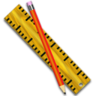
\includegraphics[width=1.5cm]{icons/distance.png}
\end{wrapfigure}
\paragraph{}
Distance mode allows to mesure the distance between two points. When the distance mode is active, all chosen models can be moved. If the user right-clicks on a model, the 2D coordinates $(u, v)$ of the clicked pixel are changed into 3D coordinates $(x, y, z)$ using OpenGL functions and a little sphere will appear at those coordinates, on the surface of the model.


\paragraph{}	
	When the two spheres are placed, a text appears at the top-right of the screen showing the distance in $cm$ between the two spheres. This distance $\delta$ between the two spheres $A(x_A, y_A, z_A)$ and $B(x_B, y_B, z_B)$ is calculated with the following formula:
\begin{align}
\delta = \sqrt{(x_A-x_B)^{2} + (y_A-y_B)^{2} + (z_A-z_B)^{2}}
\label{equ:norm}
\end{align}

\paragraph{}
	This is how this formula has been implemented with Qt functions:
	
\begin{align}
distanceBetweenTags = sqrt(pow((x_A-x_B),2) + pow((y_A-y_B),2) + pow((z_A-z_B),2))
\end{align}

``Escape'' deletes the spheres.
When the user has placed the two little spheres or performed a second click on the button, it quits the distance mode.

\paragraph{}
	Developed functions :

	\begin{code}
	OpenGLWidget -> createTags, screenToModelPixel
	\end{code}

\paragraph{}
	OpenGL functions :

	\begin{code}
	glGenLists, gluQuadricDrawStyle, glNewList, glTranslatef,

	gluSphere, glEndList, glPushMatrix, glPopMatrix, glReadPixels,

	gluUnproject
	\end{code}



\subsubsection{Rotate Model (X or Y Axis)}

\begin{wrapfigure}[3]{l}{3.5cm}
\vspace{-20pt}
\minipage{0.32\textwidth}
\includegraphics[width=1.5cm]{icons/rotateX.png}
\minipage{0.32\textwidth}
\endminipage

\includegraphics[width=1.5cm]{icons/rotateY.png}
\endminipage
\end{wrapfigure}
\paragraph{}
	A rotate model button rotates the chosen models 360° around the X or Y axis of the camera frame expressed in the model's frame for a better 3D perception of the scene without losing the manual registration.

\paragraph{}
The first step is the calculation of the rotation axis $u$ coordinates for each model. $u$ is calculated from the initial rotation matrix $R_{initial}$ derived from the model quaternion (see section~\ref{subsubsec:rotation}). That way the models will rotate around the camera frame's X or Y axis, not around their own frame's X or Y axis.


\paragraph{}
For the camera's X-axis expressed in the model's frame rotation : $u = R_{initial}^\top \left( \begin{array}{cc}
	1 \\
    0 \\
    0 \end{array} \right)$

\paragraph{}
For the camera's Y-axis expressed in the model's frame rotation : $u = R_{initial}^\top \left( \begin{array}{cc}
	0 \\
    1 \\
    0 \end{array} \right)$

Once this vector is calculated, a timer is activated to increment the rotation angle through time. Then we enter in a loop which calculates the new rotation matrix $R_{new}$ from the initial rotation matrix $R_{initial}$ for each model. This loop stops when the rotation matrix $R_{current}$ is back to its initial value $R_{initial}$. The angle $\theta$ is calculated from the timer elapsed time $t$ and the rotation speed $v$:
\begin{align}
\theta = v t
\end{align}


\paragraph{}
	At each iteration of the loop, a rotation matrix $R_{temp}$ is calculated for each model from the axis $u$ and the angle $\theta$. The new rotation matrix of each model $R_{new}$ is calculated from this temporary rotation matrix $R_{temp}$ and the initial rotation matrix $R_{initial}$. The displayed scene is then updated with the new rotation matrix $R_{new}$ applied to each model.
\begin{align}
R_{new} = R_{temp} R_{initial}
\end{align}

\paragraph{}
	Developed functions :

	\begin{code}
	OpenGLWidget -> rotateX, rotateY
	\end{code}

\paragraph{}
	Qt functions :

	\begin{code}
	QTime -> start

	QQuaternion -> fromAxisAndAngle
	\end{code}



\subsubsection{Screenshot}

\begin{wrapfigure}[2]{l}{1.5cm}
\vspace{-20pt}

\includegraphics[width=1.5cm]{icons/screenshot.png}
\end{wrapfigure}
\paragraph{}
	This button opens an explorer window for the user to select a folder and a file name. The central visual output widget display will be saved as an image file in this location.

\paragraph{}
	Developed functions :

	\begin{code}
	MainWindow -> screenshot
	\end{code}

\paragraph{}
	Qt functions :

	\begin{code}
	QImage -> grabFrameBuffer, save
	
	QFileDialog -> getSaveFileName	
	\end{code}



\subsubsection{Frame By Frame Mode}

\begin{wrapfigure}[3]{l}{1.5cm}
\vspace{-20pt}

\includegraphics[width=1.5cm]{icons/frameByFrame.png}
\end{wrapfigure}
\paragraph{}
	This mode opens two successive explorer windows for the user to select a video and a screenshot folder. The first video frame will be displayed as background image (see subsection~\ref{subsubsec:load video} for details about the video reading). Pressing the ``N'' key will display the next video frame as a background image.
	
	Pressing ``Return'' or ``Enter'' key will take a screenshot of the scene, a screenshot of the scene without models and save all the loaded models into .obj file into the screenshot folder. Then the next video frame is displayed as background image.

\paragraph{}
	Developed functions :

	\begin{code}
	OpenGLWidget -> setFrameByFrameMode, setVideoPath, updateVideo,
	
	releaseVideoCapture
	
	GLtexture -> setTexture(Mat)

	MainWindow -> screenshot
	\end{code}

\paragraph{}
	Qt functions :

	\begin{code}
	QFileDialog -> getOpenFileName

	QImage -> width, height

	QGLWidget -> convertToGLFormat
	\end{code}

\paragraph{}
	OpenCV functions :

	\begin{code}
	VideoCapture -> get(CAP\_PROP\_FPS), release

	Mat -> cvtColor, bits
	\end{code}

\paragraph{}
	OpenGL functions :

	\begin{code}
	glGenTextures, glBindTexture, glTexImage2D, glTexParameteri
	\end{code}



\subsubsection{Settings}

\begin{wrapfigure}[3]{l}{1.5cm}
\vspace{-20pt}

\includegraphics[width=1.5cm]{icons/settings.png}
\end{wrapfigure}
\paragraph{}
	This button opens the settings window. From this window the user can change translation incrementation values, camera parameters and other interface elements (see figures~\ref{settings_001}, \ref{settings_002} and \ref{settings_003}).

\vspace{10pt}
\begin{figure}[H]
\minipage{0.3\textwidth}
\centerline{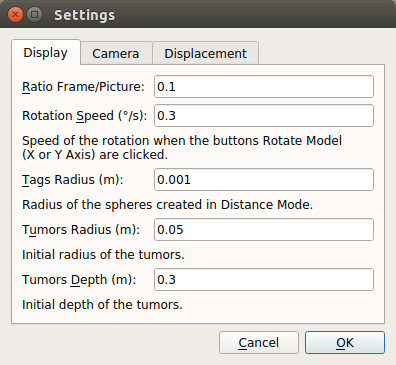
\includegraphics[scale = 0.38]{img/Settings_001.png}}
\caption{Display settings.}
\label{settings_001}
\endminipage\hfill
\minipage{0.3\textwidth}
\centerline{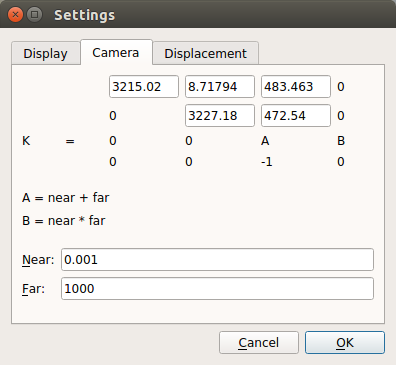
\includegraphics[scale = 0.38]{img/Settings_002.png}}
\caption{Camera settings.}
\label{settings_002}
\endminipage\hfill
\minipage{0.3\textwidth}\vspace{14pt}
\centerline{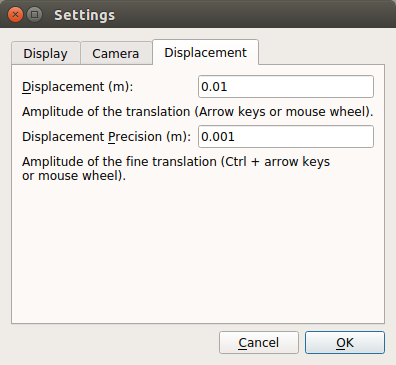
\includegraphics[scale = 0.38]{img/Settings_003.png}}
\caption{Displacement settings.}
\label{settings_003}
\endminipage
\end{figure}

\paragraph{}
	Developed functions :

	\begin{code}
	MainWindow -> settingsWindow, sendSettings
	\end{code}

\paragraph{}
	Qt functions :

	\begin{code}
	QDialog -> exec

	QLineEdit -> text
	\end{code}



\subsection{Right Toolbar Elements} \label{subsec:righy toolbar}
\paragraph{}
This subsection shows the buttons of the right toolbar. We will explain their function and implementation.

\subsubsection{Opacity Slider}

\begin{wrapfigure}[5]{l}{1cm}
\vspace{-25pt}
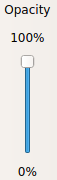
\includegraphics[width=1cm]{img/opacitySlider.png}
\end{wrapfigure}
\paragraph{}
	This slider changes the opacity of the chosen models, from 0\% to 100\%. The opacity is an OpenGL parameter which blends the color of a model with the background color. This gives a sense of the model being transparent. This transparency is a key element of the augmented reality. Indeed, by changing the liver model opacity we will be able to see its inner structures.

\paragraph{}
	Developed functions :
	\begin{code}
	
	 OpenGLWidget -> setOpacity
	\end{code}

\paragraph{}
	OpenGL functions :

	\begin{code}
	glEnable(GL\_BLEND), glBlendFunc(GL\_SRC\_ALPHA, GL\_ONE\_MINUS\_SRC\_ALPHA)
	\end{code}



\vspace{20pt}
\subsubsection{Scale Slider} \label{subsubsec:scale slider}

\begin{wrapfigure}[6]{l}{1cm}
\vspace{-25pt}
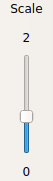
\includegraphics[width=1cm]{img/scaleSlider.png}
\end{wrapfigure}
\paragraph{}
	This slider scales the background image/video and the perspective camera from 1\% to 200\%. This is useful in case the image size is bigger than the screen size or too small. It helps to make visual output more perceptible.
The background image $width$ and $height$ are multiplied with the $scale$ factor.
The camera matrix $K$ (see formula~\ref{equ:camera parameters} for details about the camera matrix) is also scaled to display the model according to the scaled background image in order to avoid any distortion.

\begin{align}
K = \begin{pmatrix}
\alpha * scale& s * scale& u_0 * scale\\
0& \beta * scale& v_0 * scale&\\
0& 0& 1
\end{pmatrix}
\end{align}


\paragraph{}
	Developed functions :
	\begin{code}
	
	MainWindow -> scaleSliderState

	OpenGLWidget -> setCameraSettings, scaleSliderState,
	
	resizeMainWindow
	\end{code}



\vspace{10pt}
\subsubsection{Models List} \label{subsubsec:models list}

\begin{wrapfigure}[8]{l}{3cm}
\vspace{-15pt}
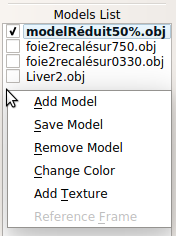
\includegraphics[width=3cm]{img/modelsList.png}
\end{wrapfigure}
\paragraph{}
	This list shows the name of all loaded models. The checkbox in the left specifies if the model is chosen or not. To activate this checkbox, the user has to left-click on it. If the user double left-click on the model name, this model will become the reference frame. If this model was the reference frame, he will not be. A right-click on a model or the void space opens a menu with shortcuts to most buttons on the left toolbar. If the click was done on a model, the action will be applied to this model only. If it was done in the void space, it will be applied to all chosen models.

\paragraph{}
	Developed functions :

	\begin{code}
	ModelsListWindow -> emitAddModel, emitSaveModels,
	
	emitRemoveModels, emitChangeColor, emitAddTexture,
	
	emitReferenceModel,	updateCheckedModels
	\end{code}

\paragraph{}
	Qt functions :

	\begin{code}
	QListWidget -> addItem, clear

	QListWidgetItem -> itemAt, checkState
	\end{code}










\vspace{10pt}
%----------------------------------------------------------------------%
\chapter{Manual Rigid Registration} \label{sec:problem} 


\section{Principle}

\paragraph{}
	Manual rigid registration is necessary to perform augmented reality during a surgery. The principle of registration is to superimpose the model with the image so that they become coincident. That way, we can assume the model to be in the same pose as the liver seen in the image. During a surgery, the laparoscope is too close to the liver to see its entire shape, we only see a small part of its surface. For this reason, an automatic registration, even with rigid model, is a very difficult problem and therefore the surgeon has to do it manually for the time being.
Another reason why this registration is hard to do is because the patient's liver is deformable and the model is rigid, so the model won't perfectly fit and the surgeon has to approximate its pose regarding the patient's deformed liver seen in the image.


\section{Testing with Users}

\subsection{Exercices}

\paragraph{}
	To improve the ergonomy of the GUI, the software has been tested by some volunteer users. The users do not work in the computer or in the medical field to eliminate as much bias as possible through their understanding of the software. For the test, they were required to do a series of registration exercises. A guidance document was provided to explain the goal of each exercice and how to do it (see appendix). The registration was done with a liver model and a picture of this model printed with a 3D printer (see figures~\ref{exercice1}, \ref{exercice3}, \ref{exercice4} and \ref{exercice5}).

\paragraph{}
	In figure~\ref{exercice1}, we can see the scene displayed in the first and second exercices. The first exercice explains how to load a background image and a model. The second one explains how to perform a registration using translations.
	
\vspace{10pt}
\begin{figure}[H]
\centerline{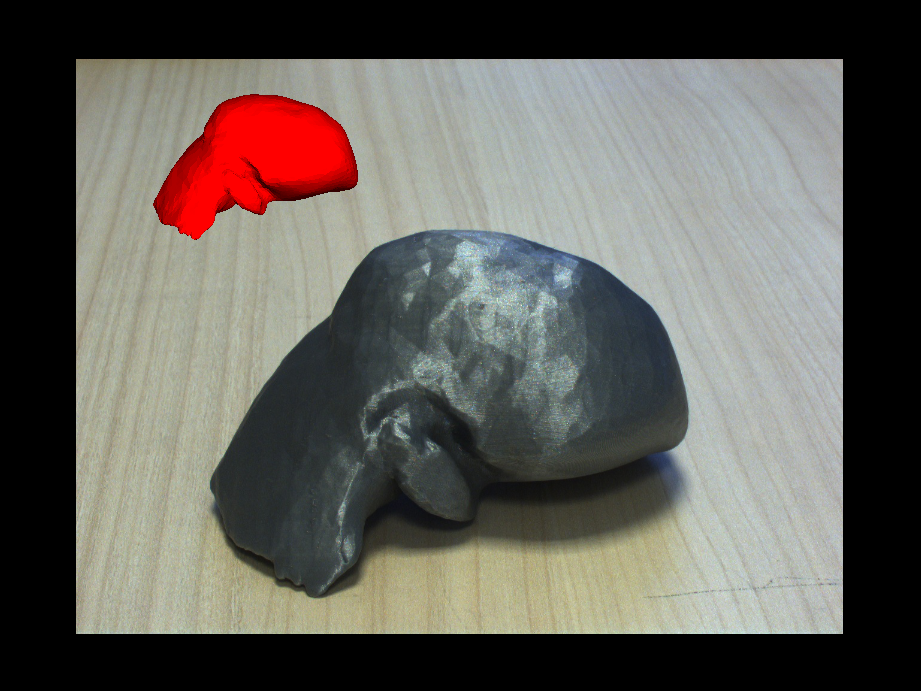
\includegraphics[scale = 0.3]{img/exercice1.png}}
\caption{GUI testing, exercices 1 and 2.}
\label{exercice1}
\end{figure}


\paragraph{}
	In figure~\ref{exercice3}, we can see the scene displayed in the third exercice. It explains how to perform a registration using rotations with the help of the opacity slider.

\vspace{10pt}
\begin{figure}[H]
\centerline{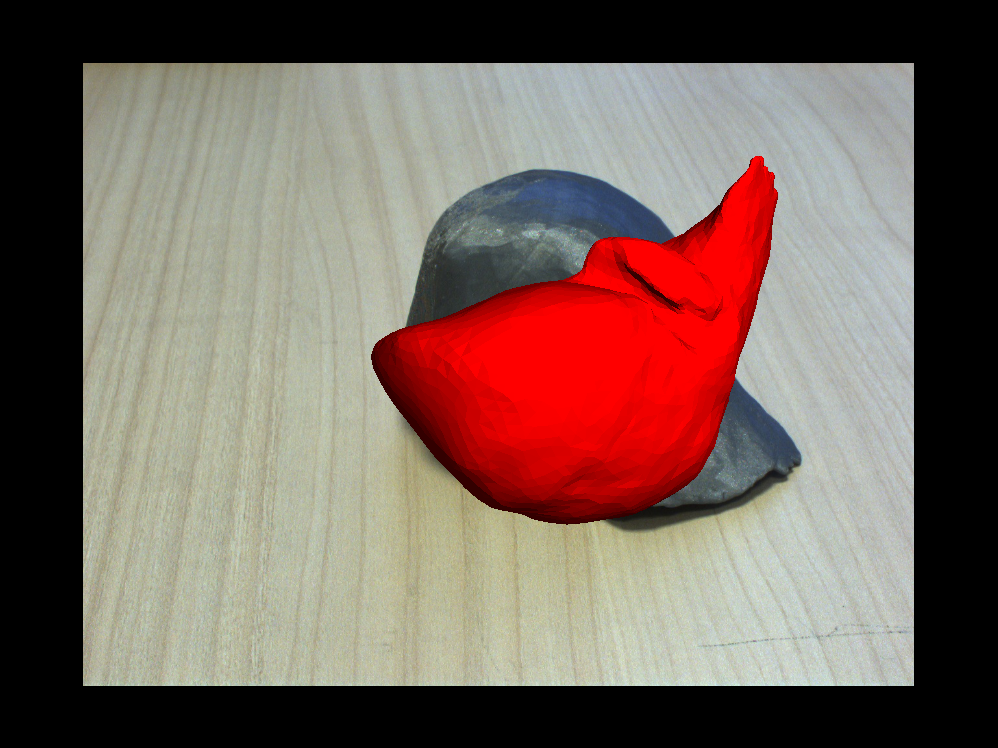
\includegraphics[scale = 0.3]{img/exercice3.png}}
\caption{GUI testing, exercice 3.}
\label{exercice3}
\end{figure}

\paragraph{}
	In figure~\ref{exercice4}, we can see the scene displayed in the fourth exercice. On this one the user have to perform a registration using rotations and translations.

\vspace{10pt}
\begin{figure}[H]
\centerline{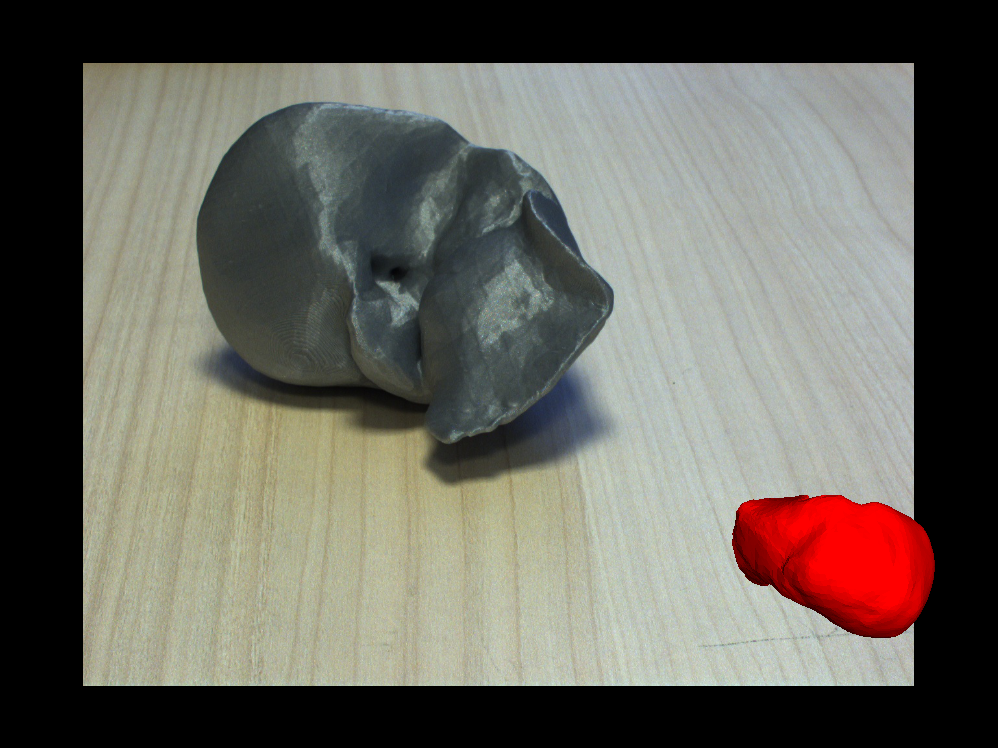
\includegraphics[scale = 0.3]{img/exercice4.png}}
\caption{GUI testing, exercice 4.}
\label{exercice4}
\end{figure}

\paragraph{}
	In figure~\ref{exercice5}, we can see the scene displayed in the fifth exercice. In this one the user has to perform a registration using rotations and translations. This exercice is harder than the previous one because the liver is obscured by itself and the visible face is smooth. At loading, the model is out of the screen and the user must click the center model button to see it.

\vspace{10pt}
\begin{figure}[H]
\centerline{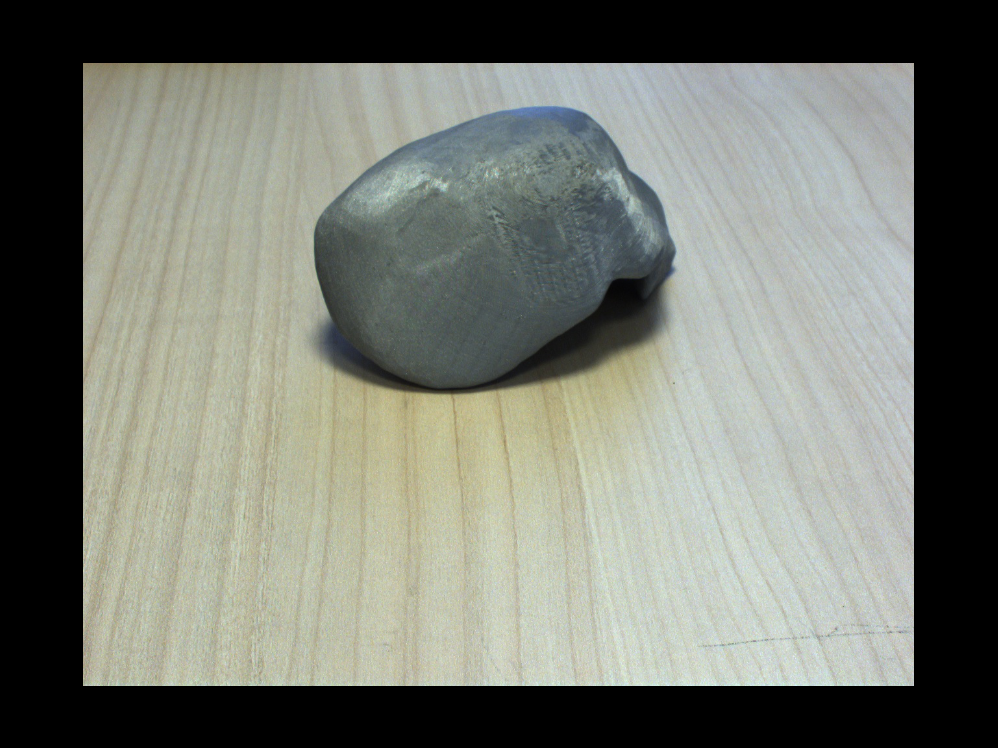
\includegraphics[scale = 0.3]{img/exercice5.png}}
\caption{GUI testing, exercice 5.}
\label{exercice5}
\end{figure}

\paragraph{}
In the end of the exercices, I asked each user if each part was difficult or easy to them. If it was difficult, then why and what do they propose to improve the GUI.


\subsection{Results}
\paragraph{}
We can see the results of those tests in the table~\ref{table}. This table shows the time spend by the users in minutes to finish each exercice. Some users have not been able to complete certain exercices because they found them too difficult. In those cases the time is replaced by the symbol ``X'' in the table:

\begin{table}[H]
\centerline{\begin{tabular}{|c|c|c|c|c|c|c|}
\hline
& Exercice 1& Exercice 2& Exercice 3& Exercice 4& Exercice 5& \textbf{Total} \\
\hline
User 1& 4& 3& X& 5& 3& \textbf{X} \\
\hline
User 2& 2& 1& 2& 6& 5& \textbf{16} \\
\hline
User 3& 4& 5& 8& X& 5& \textbf{X} \\
\hline
User 4& 1& 4& 5& X& 2& \textbf{X}\\
\hline
User 5& 4& 4& 7& 8& 6& \textbf{29} \\
\hline
\textbf{Average}& \textbf{3}& \textbf{3.4}& \textbf{5.5}& \textbf{6.3}& \textbf{4.2}& \textbf{22.5} \\
\hline
\end{tabular}}
\caption{GUI testing results.}
\label{table}
\end{table}

\paragraph{}
The observations shows a fast adaptation to the software. I tried to understand what features were good or had to be improved on the GUI according to what users said and to my observations:
\begin{itemize}
\item They learned the keys very fast. After the second exercice, all the users were able to use the control keys without looking at the keyboard and mouse, except for the ``Ctrl'' button.
\item They had no problem with the use of the opacity slider and the 360° rotate buttons and quickly understood their usefulness.
\item They did not have any problems to open and change models or background images except for one tester who tried to drag and drop an image file onto the GUI to open it. This is a good idea which has to be implemented for the images/videos and for the .obj models as well.
\item They had a poor sense of depth in the software GUI. This problem was known since the beginning of the development. However I noticed they had almost never consult the model depth at the top-right of the screen. Maybe we have to make it more visible.
\item They confused model size and perspective projection of depth. For example it was asked to me several times how to enlarge the model because it seemed too small to fit the image.
\item The translations part were easy, but the rotations were more complicated to perform. Maybe we can change the rotation angle equation to be more ergonomic if the problem is significant with a larger number of testers (see formula~\ref{equ:angle}, page~\pageref{equ:angle}).
\item Sometimes they were lost with the GUI buttons. Maybe we have to change the icons to make them easier to understand and to reorganize them by frequency of use for example.
\item They didn't understand how the model list in the right toolbar was working. Maybe we have to add an exercice with several models to show how it can be used. One of the tester tried to double left-click on a model in the list to active it instead of checking the box. This is a good idea implemented after the tests.
\end{itemize}



%----------------------------------------------------------------------
\chapter{Augmented Reality on Liver} \label{sec:method} 

\paragraph{}
	Augmented reality is defined as the superimposition of computerized objects into real world (Tom Caudell and David Mizell, 1992). To superimpose a virtual and a real image is easy. The main difficulty in augmented reality is to place and dimension a virtual object into real world. In this software, the object dimension is given by the perspective projection applied on the scene and its position is chosen by the user when he applies transformations to the models.

\paragraph{Augmented reality on a 3D printed liver:}
	Figures~\ref{opaquemodelPLA},~\ref{transparentmodelPLA} and~\ref{fullytransparentmodelPLA} below are screenshots from the software showing augmented reality on liver model obtained from 3D printing in polylactic acid (PLA). The software interface displays the printed liver as the background, the liver model in red and a fake tumor model represented by a sphere in blue. Those three images represents the same scene with an opacity gradient of the liver model. From left to right, the opacity of this model is reduced from $100\%$ to $0\%$. That way we see the tumor inside the liver model and the scene behind it. The registration only took me about one minute because the PLA liver is rigid and we see it entirely.

\begin{figure}[H]
\minipage{0.3\textwidth}
\centerline{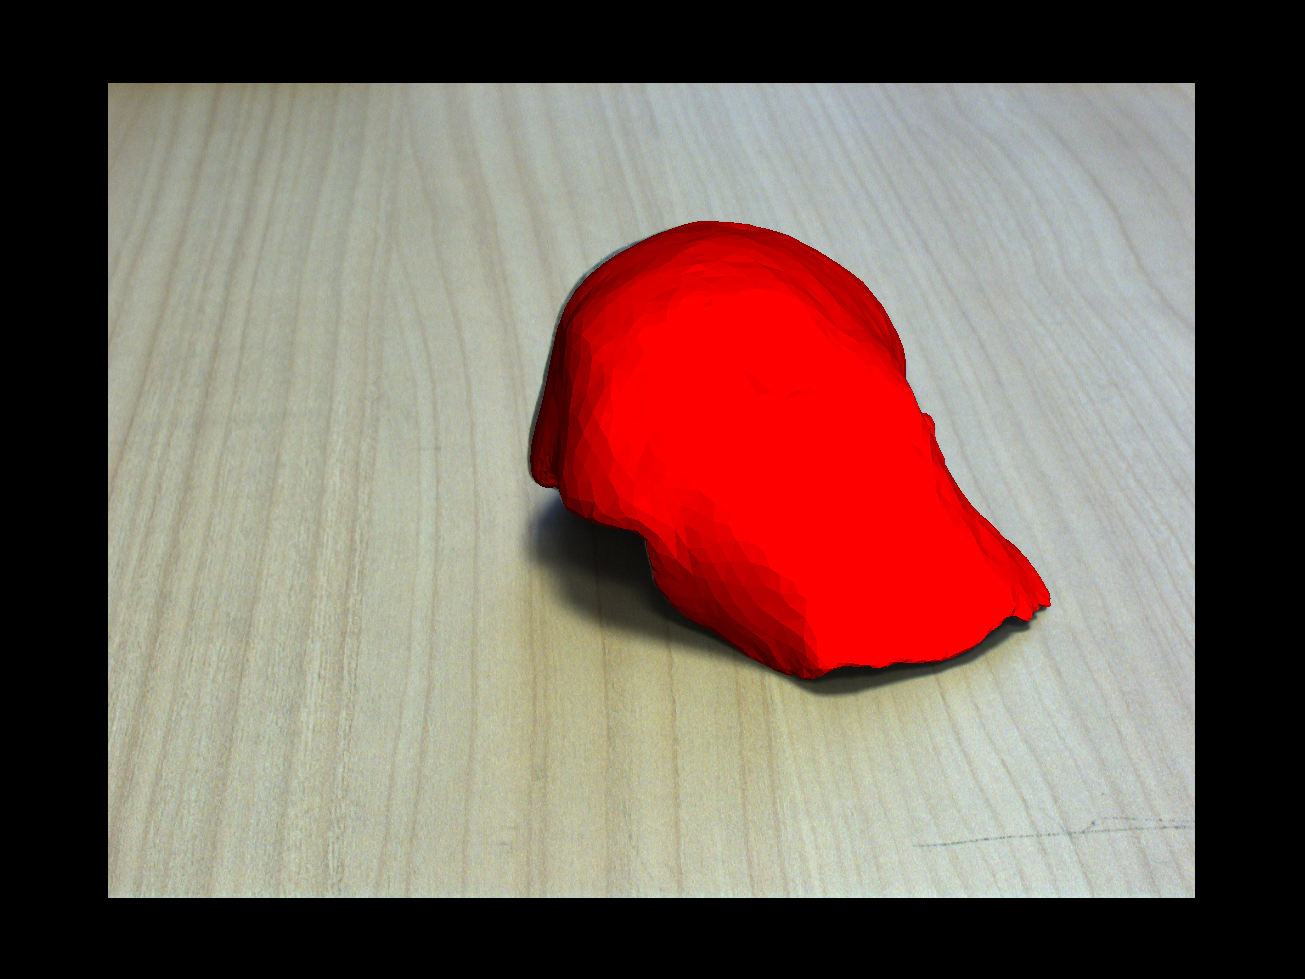
\includegraphics[scale = 0.2]{img/PLAimage_1.png}}
\caption{Augmented reality with opaque model on a 3D printed liver.}
\label{opaquemodelPLA}
\endminipage\hfill
\minipage{0.3\textwidth}
\centerline{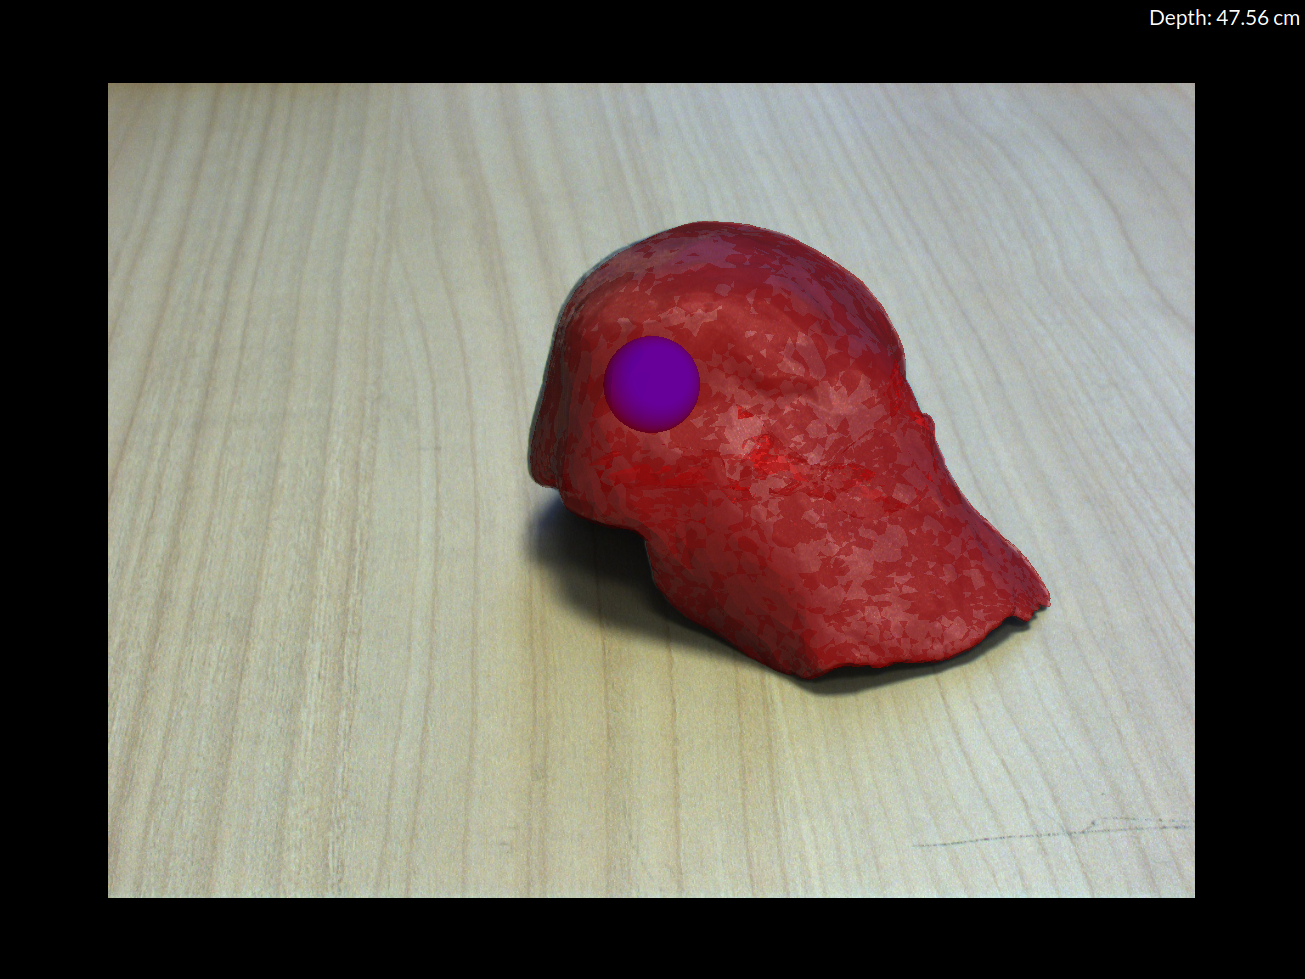
\includegraphics[scale = 0.2]{img/PLAimage_2.png}}
\caption{Augmented reality with partially transparent model on a 3D printed liver.}
\label{transparentmodelPLA}
\endminipage\hfill
\minipage{0.3\textwidth}
\centerline{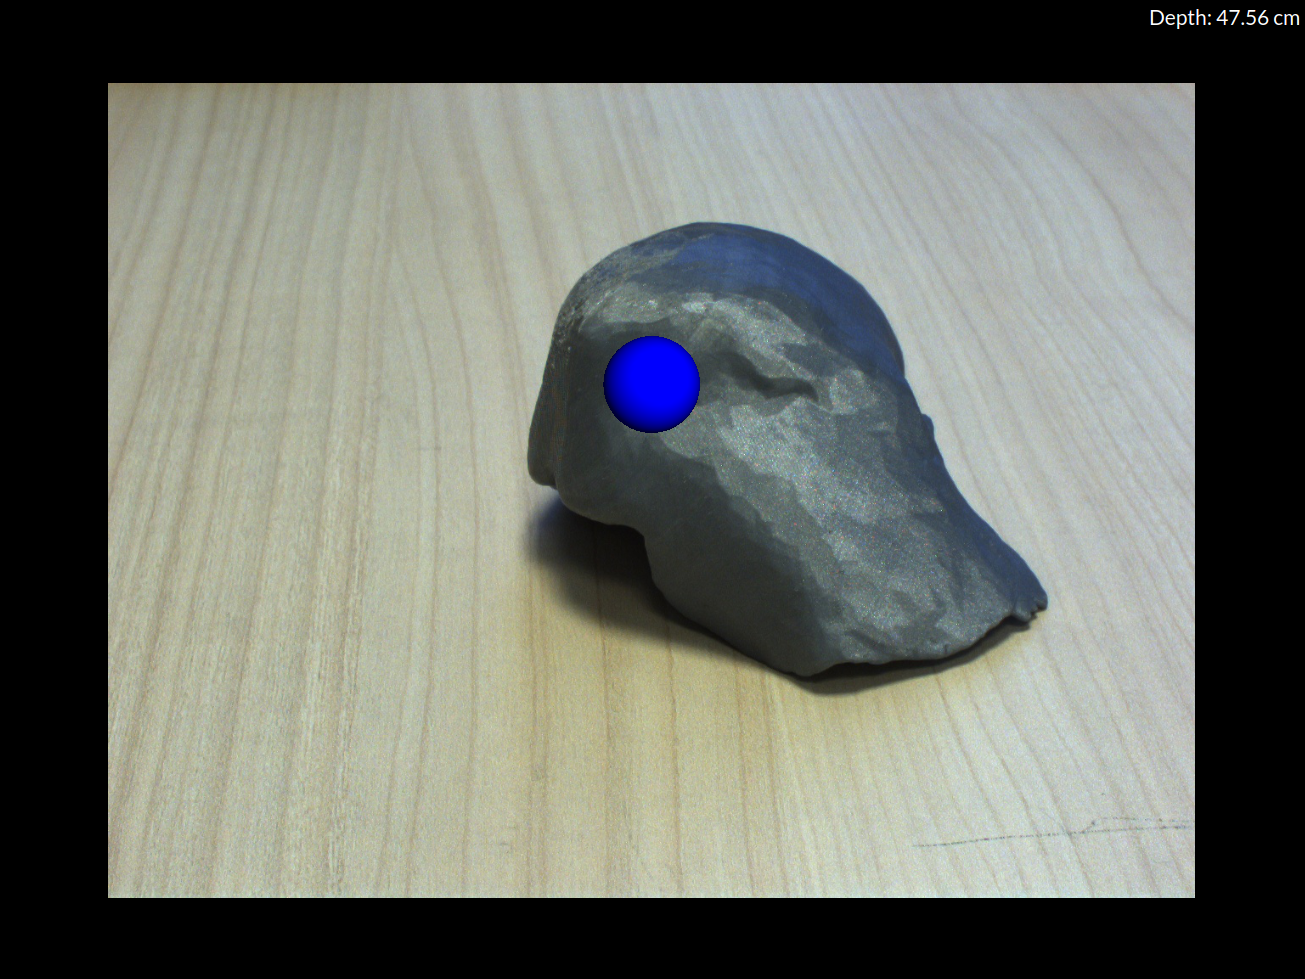
\includegraphics[scale = 0.2]{img/PLAimage_3.png}}
\caption{Augmented reality with fully transparent model on a 3D printed liver.}
\label{fullytransparentmodelPLA}
\endminipage
\end{figure}


\paragraph{Augmented reality on a patient's liver:}
	Figures~\ref{opaquemodel} and~\ref{transparentmodel} below are screenshots from the software showing augmented reality on a surgical scene obtained from a liver surgery. The software interface displays the surgical scene as the background, the liver model in red and a tumor model in white. The black area around the scene is here to show the entire liver model because the image displayed by the laparoscope covers only a part of the liver. We left the liver opaque on the left image to show the registration but it can easily be made fully transparent to prevent it from disturbing the surgeon. On the right image the liver is partially transparent so we can see the tumor inside, the patient's liver behind and still be sure the liver model is well registered.


\begin{figure}[H]
\minipage{0.4\textwidth}
\centerline{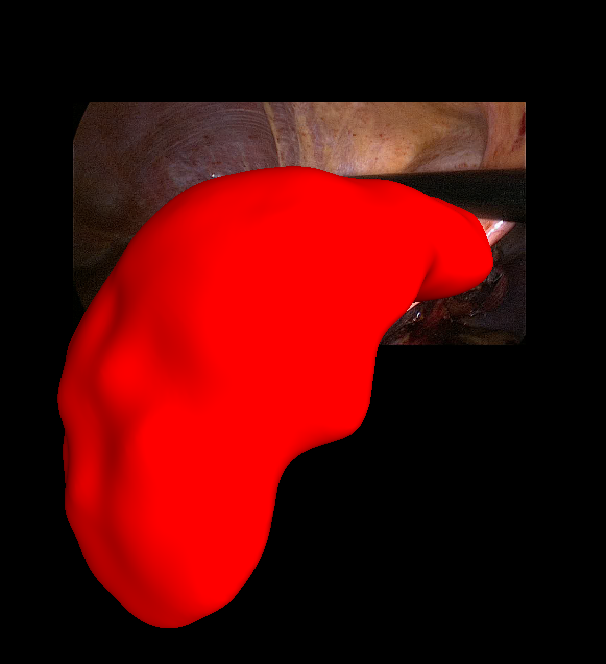
\includegraphics[scale = 0.5]{img/image_2.png}}
\caption{Augmented reality with opaque model on a patient's liver.}
\label{opaquemodel}
\endminipage\hfill
\minipage{0.45\textwidth}
\centerline{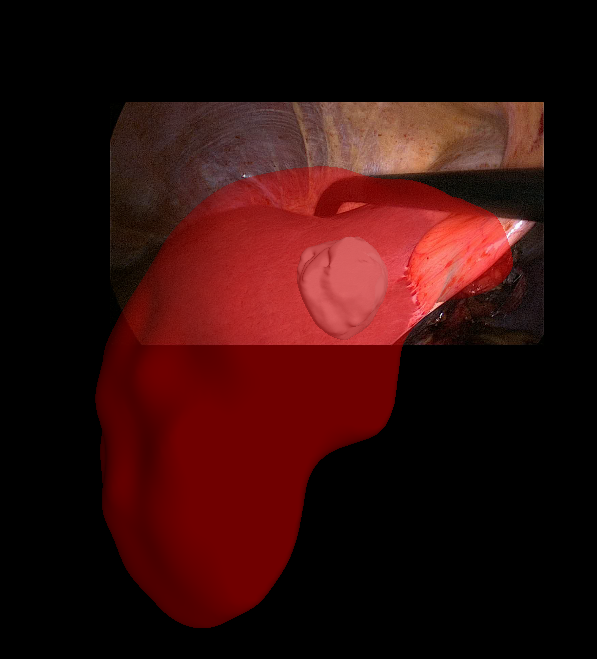
\includegraphics[scale = 0.5]{img/image_1.png}}
\caption{Augmented reality with transparent model on a patient's liver.}
\label{transparentmodel}
\endminipage
\end{figure}

\paragraph{}
 Once the liver model manually registered, the tumor model will be as well correctly aligned on the patient's liver. This helps the surgeon to gain time and accuracy. We can see that the liver model does not register properly with the patient's liver because the liver is deformed with a tool. To adress this problem, we have to make the model deformable in the future.
 

%----------------------------------------------------------------------%
\chapter{Conclusion} \label{sec:conclusion} 
\paragraph{}
The goal of this internship was to begin the developement of the software. This includes the realisation of a functional and ergonomic GUI. This GUI must allow the user to easily perform manual registrations for augmented reality. For now the software can load 3D rigid models, transform and render them over an image or video background to perform augmented reality. The basic features of the GUI have been tested with users. Those tests showed that some features need to be improved while the main ones are already functional.

\paragraph{}
I think that further testing should be performed including each software feature. Regarding the manual registration part, it is functional but only with rigid models. At this point the models have to be deformable to adapt the position of their inner structures in real-time during the surgery. I partly worked on the deformable models theory but I did not have sufficient time to implement this part during my internship. The next intern will continue to develop and implement the remaining objectives. As suggested by Bertrand Le Roy, it would also be interesting to ``cut'' the liver model to reproduce at best the influence of the surgeon's actions on the liver and keep the registration. Then the registration and the deformability have to be made automatically by the software in order for the surgeon to gain time during the surgery.



%------------------------------------------------------------------------------------------------------------------%

\begin{appendices}
\setcounter{secnumdepth}{0}

\section{GUI Testing Exercices} \label{secAppendix:A}
\paragraph{}
Le but de cette série d'exercices est d'évaluer l'ergonomie du logiciel HEPATAUG. Pour cela il vous sera demandé d'effectuer des recalages, consistant à superposer un modèle de foie avec des photos de ce même modèle réalisé par imprimante 3D.
Toutes les photos nécessaires à la réalisation de ces exercices se trouvent dans le répertoire ``Photos'' du dossier ``Ressources'', les modèles sont dans le répertoire ``Modèles'' du dossier ``Ressources''.

\paragraph{}
Pour effectuer des transformations sur le modèle, les contrôles sont les touches directionnelles du clavier et la roue de la souris pour les translations (la touche ``Ctrl'' peut être pressée simultanément pour une translation plus fine) et le ``glisser-déposer'' avec la souris pour la rotation.

\paragraph{Exercice n°1 :}Charger un modèle et une image
\begin{itemize}
\item Lancer le programme HEPATAUG.
\item Charger la photo ``Photo 1.jpg'' en cliquant sur l’icône ``Load Image'' (voir Illustration~\ref{picture}).
\item Charger le modèle ``Modèle 1.obj'' en cliquant sur l’icône ``Load Model'' (voir Illustration~\ref{model}).
\end{itemize}

\begin{figure}[H]
\minipage{0.5\textwidth}
\centerline{\includegraphics[scale = 0.9]{img/icons/picture.jpg}}
\caption{Charger une image.}
\label{picture}
\endminipage\hfill
\minipage{0.5\textwidth}
\centerline{
\includegraphics[scale = 1.4]{img/icons/load.png}}
\caption{Charger un modèle.}
\label{model}
\endminipage
\end{figure}

\begin{figure}[H]
\minipage{0.5\textwidth}
\centerline{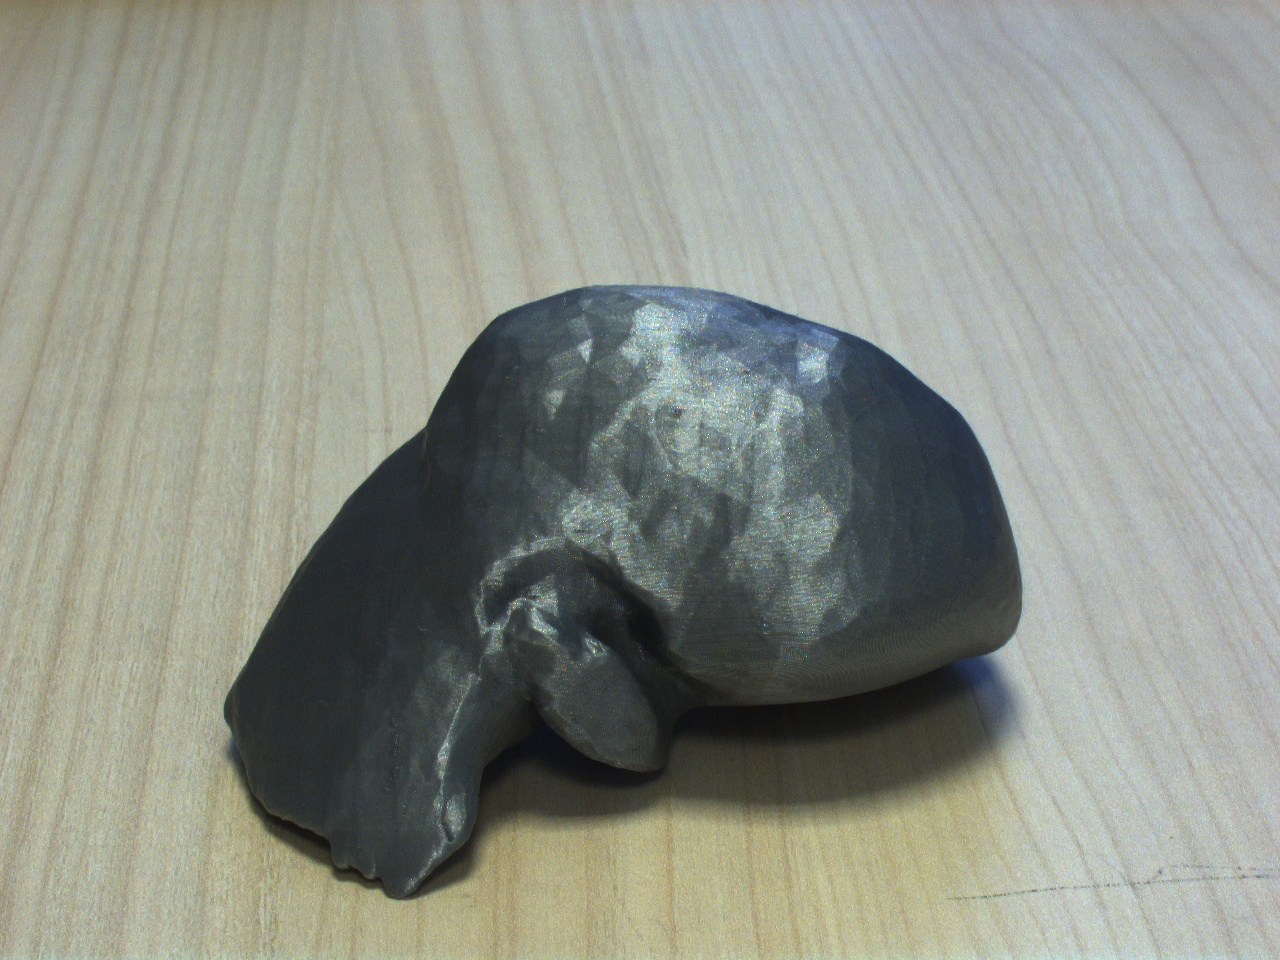
\includegraphics[scale = 0.1]{img/Photo1.jpg}}
\caption{Photo 1.}
\endminipage\hfill
\minipage{0.5\textwidth}
\centerline{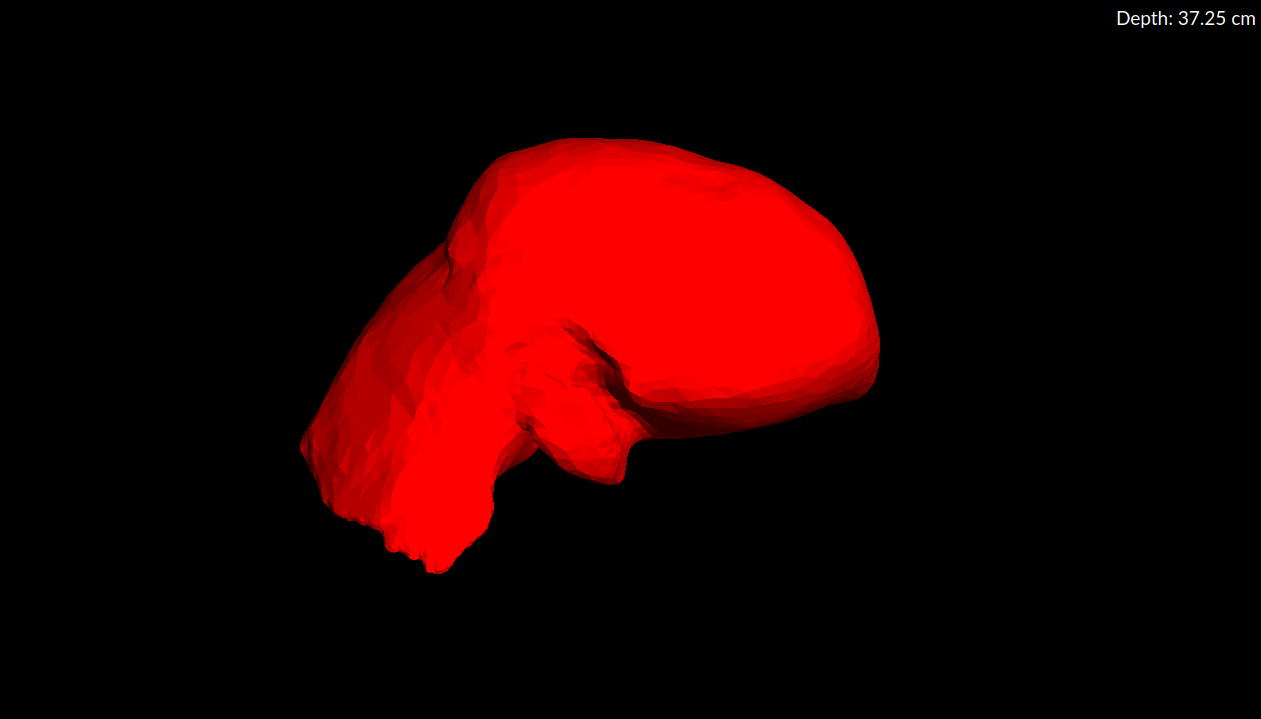
\includegraphics[scale = 0.17]{img/Model1.png}}
\caption{Modèle 1.}
\endminipage
\end{figure}

\paragraph{Exercice n°2 :}Translations
\begin{itemize}
\item Cocher la case en face du nom du modèle dans la liste de droite pour le rendre actif.
\item Recaler le modèle avec l'image en effectuant des translations grâce au pavé directionnel du clavier et à la roue de la souris. Ces translations peuvent être réalisées de façon plus précise en maintenant la touche ``Ctrl'' enfoncée.
\item La valeur du slider ``Opacity'' présent dans la barre d'outils située à droite peut être modifiée afin de vérifier visuellement si le recalage est bon (voir Illustration~\ref{opacity}).
\end{itemize}
	
\begin{figure}[H]
\minipage{0.5\textwidth}
\centerline{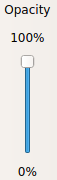
\includegraphics[scale = 0.5]{img/opacitySlider.png}}
\caption{Modifier l'opacité du modèle.}
\label{opacity}
\endminipage\hfill
\minipage{0.5\textwidth}
\centerline{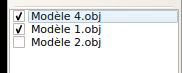
\includegraphics[scale = 1]{img/modelsListExercices.png}}
\caption{Liste des modèles.}
\label{list}
\endminipage
\end{figure}
		
\paragraph{Exercice n°3 :}Rotations
\begin{itemize}
\item Charger la photo ``Photo 2.jpg''.
\item Supprimer le modèle ``Modèle 1.obj'' en effectuant un clic droit sur le nom du modèle dans la liste de droite, puis en cliquant sur ``Remove Model''.
\item Charger le modèle ``Modèle 2.obj'' et le rendre actif comme vu précédemment.
\item Recaler le modèle avec l'image en effectuant des rotations. Il suffit pour cela de cliquer à l'aide du bouton gauche de la souris puis de la déplacer tout en maintenant le bouton appuyé.
\item Le curseur Opacity ainsi que les boutons de rotation peuvent être utilisés afin de vérifier visuellement si le recalage est bon (voir Illustrations~\ref{rotateX},\ref{rotateY}).
\end{itemize}
						

\begin{figure}[H]
\minipage{0.5\textwidth}
\centerline{\includegraphics[scale = 1]{img/icons/rotateX.png}}
\caption{Rotation de 360° selon l'axe X.}
\label{rotateX}
\endminipage\hfill
\minipage{0.5\textwidth}
\centerline{\includegraphics[scale = 1]{img/icons/rotateY.png}}
\caption{Rotation de 360° selon l'axe Y.}
\label{rotateY}
\endminipage
\end{figure}

\begin{figure}[H]
\minipage{0.5\textwidth}
\centerline{\includegraphics[scale = 0.1]{img/Photo2.jpg}}
\caption{Photo 2.}
\endminipage\hfill
\minipage{0.5\textwidth}
\centerline{\includegraphics[scale = 0.22]{img/Model2.png}}
\caption{Modèle 2.}
\endminipage
\end{figure}

\paragraph{Exercice n°4 :}Entraînement
\begin{itemize}
\item Charger la photo ``Photo 3.jpg''.
\item Supprimer le modèle ``Modèle 2.obj''.
\item Charger le modèle ``Modèle 3.obj'' et le rendre actif.
\item Recaler le modèle avec l'image en effectuant des translations et des rotations à l'aide des méthodes décrites précédemment.
\item Sauvegarder le modèle sous le nom ``Mon Modèle.obj'' dans le répertoire ``Modèles'' en effectuant un clic droit sur le modèle dans la liste puis en cliquant sur le bouton ``Save Model'' (voir Illustration~\ref{save}).
\end{itemize}


\begin{figure}[H]
\centerline{\includegraphics[scale = 0.8]{img/icons/save.png}}
\caption{Sauvegarder le modèle.}
\label{save}
\end{figure}

\begin{figure}[H]
\minipage{0.5\textwidth}
\centerline{\includegraphics[scale = 0.1]{img/Photo3.jpg}}
\caption{Photo 3.}
\endminipage\hfill
\minipage{0.5\textwidth}
\centerline{\includegraphics[scale = 0.22]{img/Model3.png}}
\caption{Modèle 3.}
\endminipage
\end{figure}

\paragraph{Exercice n°5 :}Exercice plus difficile
\begin{itemize}
\item Charger la photo ``Photo 4.jpg''.
\item Supprimer le modèle ``Modèle 3.obj''.
\item Charger le modèle ``Modèle 4.obj''. Le modèle devrait apparaître en dehors de la zone visible.
\item Centrer le modèle sur l'écran grâce au bouton ``Center Model'' (voir Illustration~\ref{center}).
\item Recaler le modèle avec l'image en effectuant des translations et des rotations à l'aide des méthodes décrites précédemment.
\end{itemize}

\begin{figure}[H]
\centerline{\includegraphics[scale = 0.8]{img/icons/center.png}}
\caption{Centrer le modèle.}
\label{center}
\end{figure}

\begin{figure}[H]
\minipage{0.5\textwidth}
\centerline{\includegraphics[scale = 0.1]{img/Photo4.jpg}}
\caption{Photo 4.}
\endminipage\hfill
\minipage{0.5\textwidth}
\centerline{\includegraphics[scale = 0.22]{img/Model4.png}}
\caption{Modèle 4.}
\endminipage
\end{figure}


\end{appendices}


\begin{thebibliography}{2}
\expandafter\ifx\csname natexlab\endcsname\relax\def\natexlab#1{#1}\fi

\bibitem[Simek 2013]{}
Simek K., Calibrated Cameras In Opengl Without Glfrustum,
\newblock \textit{Ksimek.github.io}, Web. 18 Aug. 2016.

\bibitem[Shoemake 1985]{}
Shoemake K., Computer Graphics 19(3):245-254
\newblock \textit{Dl.acm.org}, Web. 18 Aug. 2016.


\bibitem[Nebra 2015]{}
Nebra M., Schaller M., Programmez avec le langage C++,
\newblock \textit{Openclassrooms.com}, Web. 18 Aug. 2016.

\bibitem[Kayl 2013]{}
Kayl, Créez des programmes en 3D avec OpenGL,
\newblock \textit{Openclassrooms.com}, Web. 18 Aug. 2016.

\bibitem[Gauthier 2015]{}
Gauthier M., Gérer son code avec Git et GitHub,
\newblock \textit{Openclassrooms.com}, Web. 18 Aug. 2016.


\bibitem[Haubold 2015]{}
Haubold L., Grant, T., Nehe OpenGL tutorials,
\newblock \textit{Nehe.gamedev.net}, Web. 18 Aug. 2016.

\bibitem[Cuvelier 2016]{}
Cuvelier T., Club des professionnels en informatique,
\newblock \textit{Developpez.com}, Web. 18 Aug. 2016.

\bibitem[Qt organization 2016]{}
N.p., Qt Documentation,
\newblock \textit{Doc.qt.io}, Web. 18 Aug. 2016.

\bibitem[OpenGL.org organization 2016]{}
OpenGL.org organization, OpenGL Software Development Kit Documentation,
\newblock \textit{Opengl.org/sdk/docs}, Web. 18 Aug. 2016.

\bibitem[OpenCV.org organization 2016]{}
OpenGL.org organization, OpenCV: cv Namespace Reference,
\newblock \textit{Docs.opencv.org/3.1.0/d2/d75/namespacecv.html}, Web. 18 Aug. 2016.
\end{thebibliography}
\end{document}
